\documentclass[11pt,a4paper]{article}
\usepackage[utf8]{inputenc}
\usepackage[T1]{fontenc}
\usepackage[spanish]{babel}
\usepackage[margin=2.5cm]{geometry}
\usepackage{parskip}
\usepackage{hyperref}
\usepackage{enumitem}
\usepackage{booktabs}
\usepackage{array}
\usepackage{xcolor}
\usepackage{graphicx}
\usepackage{longtable}
\usepackage{amsmath}
\usepackage{amssymb}

\definecolor{done}{RGB}{0,140,0}
\definecolor{partialcol}{RGB}{200,120,0}
\definecolor{pendingcol}{RGB}{180,0,0}
\definecolor{bugcol}{RGB}{140,0,140}

\setlength{\parindent}{0pt}
\setlength{\parskip}{6pt}

\hypersetup{colorlinks=true, linkcolor=black, urlcolor=blue}

\title{\textbf{Búsqueda Inteligente de Objetos en Simulación}\\
\large Estado actual del proyecto y plan de implementación\\
\normalsize Detección (YOLOE) + Búsqueda (VLMaps) + Navegación (Habitat-Sim)\\
Extensión: ROS 1 Noetic + Toyota HSR}
\author{Mario García Blasco}
\date{8 de junio de 2026}

\begin{document}

\maketitle
\tableofcontents
\newpage

% ─────────────────────────────────────────────────────────────────────────────
\section{Visión general del proyecto}
% ─────────────────────────────────────────────────────────────────────────────

\subsection{Problema}

Dado un objetivo expresado en lenguaje natural (por ejemplo, \textit{"find the laptop"}), un robot
simulado debe localizar el objeto de forma eficiente en un entorno interior. El robot opera en
escenas Matterport3D y HSSD renderizadas con Habitat-Sim.

\subsection{Hipótesis}

Un sistema que combine tres niveles de conocimiento --- etiquetas de habitaciones, memoria
semántica de mobiliario (VLMaps, 37 categorías MP3D / 36 categorías HSSD) y verificación
visual de vocabulario abierto (YOLOE) --- encuentra objetos específicos de forma más eficiente
que métodos que dependen de un solo nivel.

\subsection{Los tres niveles de conocimiento}

\begin{center}
\begin{tabular}{lll}
\toprule
\textbf{Nivel} & \textbf{Herramienta} & \textbf{Qué sabe} \\
\midrule
Habitación & LabelMe (MP3D) / \texttt{semantic\_config.json} (HSSD) &
  «Esto es el salón» \\
Mueble / zona & VLMaps (37 cats MP3D / 36 cats HSSD) &
  «Hay un sofá allí» \\
Objeto específico & YOLOE (open-vocab) &
  «Hay un portátil encima de esa mesa» \\
\bottomrule
\end{tabular}
\end{center}

\subsection{Idea clave: VLMaps estrecha la búsqueda, YOLOE confirma}

\begin{enumerate}
  \item El usuario pide un objeto específico («laptop»).
  \item Un LLM traduce ese objeto a categorías VLMap donde es probable encontrarlo:
        \texttt{laptop} $\rightarrow$ \texttt{[table, counter, shelving]}.
  \item VLMaps localiza todas las instancias de esas categorías en el mapa.
  \item El robot navega al candidato más prometedor.
  \item YOLOE mira con la cámara y confirma si el objeto está ahí.
  \item Si no $\rightarrow$ siguiente candidato. Si sí $\rightarrow$ \textbf{ENCONTRADO}.
\end{enumerate}

\subsection{Etiquetado de habitaciones}

Para instrucciones del tipo \textit{"go to the living room and find the laptop"}, el robot
necesita saber dónde está el salón.

\begin{itemize}
  \item \textbf{MP3D}: etiquetado manual offline con LabelMe (pipeline lista, pendiente de ejecutar).
  \item \textbf{HSSD}: anotaciones nativas en \texttt{semantics/scenes/<id>.semantic\_config.json}.
        La clase \texttt{SemanticSceneRoomProvider} las rasteriza sobre el grid del VLMap sin
        necesidad de LabelMe.
\end{itemize}

% ─────────────────────────────────────────────────────────────────────────────
\section{Estado actual del proyecto (15 mayo 2026)}
% ─────────────────────────────────────────────────────────────────────────────

\subsection{Infraestructura --- \textcolor{done}{COMPLETADA}}

\begin{itemize}
  \item[\checkmark] Docker con CUDA 12.1 + Habitat-Sim 0.3.1 + conda (Python 3.9)
  \item[\checkmark] 3 escenas MP3D con VLMaps construidos:
        \textbf{gTV8FGcVJC9\_1}, \textbf{jh4fc5c5qoQ\_1}, \textbf{mJXqzFtmKg4\_1}
  \item[\checkmark] 4 escenas adicionales descargadas (sin VLMap aún):
        mJXqzFtmKg4, jh4fc5c5qoQ, JeFG25nYj2p, Uxmj2M2itWa
  \item[\checkmark] 1 escena HSSD integrada: \textbf{102344280} (15 habitaciones, $\sim$447 m²),
        VLMap construido e indexado
  \item[\checkmark] Menú interactivo en Docker (\texttt{menu.sh}) para toda la pipeline
  \item[\checkmark] Submodule git \texttt{third\_party/vlmaps} (rama \texttt{tfg-modifications})
  \item[\checkmark] Repositorio limpio en GitHub: \texttt{mobileclip\_blt.ts} (571 MB) eliminado
        del historial con \texttt{git-filter-repo}; push operativo
\end{itemize}

\subsection{Navegación interactiva --- \textcolor{done}{COMPLETADA}}

\begin{itemize}
  \item[\checkmark] Pipeline completa: instrucción $\rightarrow$ LLM $\rightarrow$ goal selection
        $\rightarrow$ visgraph $\rightarrow$ navegación live con visualización
  \item[\checkmark] \texttt{plan\_path\_only()}: planificación sin ejecución --- elimina el
        teletransporte; camino mostrado como línea roja 800 ms antes de ejecutar
  \item[\checkmark] Movimientos lentos y fluidos (\texttt{\_NAV\_STEP\_DELAY\_MS = 80 ms})
  \item[\checkmark] Dirección de cara corregida:
        $\theta = \arctan2(-\Delta y, -\Delta x)$, signo de giro consistente con el
        planificador interno
  \item[\checkmark] Goal selection con 3 niveles de fallback (room centroid / BFS / heatmap peak)
  \item[\checkmark] Visgraph con margen de 4 px ($\sim$20 cm); recuperación de colisión
        (giro $30^\circ$ + avance + replanificación); hasta 3 replanes y 8 candidatos
  \item[\checkmark] Heatmap semántico overlay (JET colormap, 50\% opacidad)
  \item[\checkmark] Cámara primera persona con inclinación $-30^\circ$
  \item[\checkmark] Multi-goal retry (hasta 8 candidatos por categoría, ordenados por BFS)
\end{itemize}

\subsection{Mapper LLM --- \textcolor{done}{COMPLETADO}}

\begin{itemize}
  \item[\checkmark] El LLM traduce objetos no-VLMap a categorías VLMap probables.
        Ejemplo: \texttt{laptop} $\rightarrow$ \texttt{[table, counter, shelving]}
  \item[\checkmark] Distingue queries directas (\texttt{sofa} $\in$ MP3D) e indirectas
        (\texttt{laptop} $\notin$ MP3D)
  \item[\checkmark] Room-based reasoning: sugiere habitaciones probables además de muebles.
        Ejemplo: \texttt{laptop} $\rightarrow$ \texttt{rooms: [office, bedroom]}
  \item[\checkmark] Prompt con 6 few-shot examples incluyendo rooms
\end{itemize}

\subsection{Siguiente extensión semántica antes de ROS --- objetos no-VLMap abiertos}

\textbf{Decisión táctica (24 abril 2026).} Antes de migrar el proyecto a ROS 1
Noetic conviene estabilizar una capa semántica más rica para \textbf{objetos
específicos que ya aparecen en HSSD pero no forman parte del vocabulario base
de VLMaps}. Esto permite validar la parte difícil del problema
\emph{semántico-visual} antes de mezclarla con problemas de ROS, Gazebo,
\texttt{tf}, \texttt{move\_base} o el HSR.

\paragraph{Tesis de diseño.} El mapeo
\texttt{objeto específico $\rightarrow$ muebles surrogate} no debe quedarse en
una tabla manual cerrada. Para objetos como \texttt{bottle},
\texttt{charger}, \texttt{notebook} o \texttt{printer}, el sistema debe ser
capaz de inferir dónde buscar sin tener que añadir una regla nueva cada vez.
Por eso:
\begin{itemize}
  \item el \textbf{LLM} debe decidir el \emph{target canónico}, una lista
        ordenada de muebles surrogate y, opcionalmente, habitaciones probables;
  \item una \textbf{capa de validación determinista} debe filtrar esa salida y
        quedarse solo con categorías VLMap realmente navegables;
  \item \texttt{object\_priors.py} debe mantenerse como \textbf{fallback
        auditado}, no como única fuente de decisión.
\end{itemize}

\paragraph{Shortlist aprobada para la siguiente sesión.}
\begin{itemize}
  \item \textbf{Prioridad alta}: \texttt{laptop}, \texttt{book},
        \texttt{soap}, \texttt{vase}, \texttt{candle}.
  \item \textbf{Prioridad media}: \texttt{basket}, \texttt{printer},
        \texttt{teapot}.
\end{itemize}

\paragraph{Flujo objetivo.} Para targets fuera del vocabulario VLMap:
\begin{enumerate}
  \item \textbf{Normalización léxica}: resolver aliases triviales
        (\texttt{computer}$\rightarrow$\texttt{laptop},
        \texttt{books}$\rightarrow$\texttt{book},
        \texttt{tea pot}$\rightarrow$\texttt{teapot},
        \texttt{soap dispenser}$\rightarrow$\texttt{soap}).
  \item \textbf{Consulta al LLM}: pedir una salida estructurada con
        \texttt{canonical\_target}, \texttt{query\_mode},
        \texttt{surrogate\_categories}, \texttt{likely\_rooms},
        \texttt{yoloe\_label} y \texttt{aliases}.
  \item \textbf{Validación}: filtrar los surrogates contra
        \texttt{get\_categories("hssd")} y contra el vocabulario realmente
        disponible en la escena.
  \item \textbf{Planificación}: construir el heatmap con los muebles surrogate
        supervivientes.
  \item \textbf{Verificación}: YOLOE confirma el
        \texttt{canonical\_target}, no el surrogate. Es decir, se navega a una
        \texttt{table} o a un \texttt{desk}, pero se verifica
        \texttt{laptop}.
\end{enumerate}

\paragraph{Objetivo práctico.} La salida del LLM debe responder a
\emph{qué objeto es} y \emph{sobre qué tipo de mueble conviene buscarlo}; el
sistema debe seguir controlando \emph{qué parte de esa sugerencia es
ejecutable}. Esto deja el camino preparado para búsquedas más abiertas de nivel
3 y para una posterior migración a ROS con una semántica ya endurecida.

\subsection{YOLOE como verificador --- \textcolor{done}{COMPLETADO}}

\begin{itemize}
  \item[\checkmark] Worker persistente (\texttt{\_yoloe\_persistent\_worker.py}): modelo
        cargado una sola vez; inferencias $\sim$100--500 ms en lugar de $\sim$30 s
  \item[\checkmark] Protocolo stdout correcto: diagnósticos a \texttt{sys.stderr},
        \texttt{start()} lee hasta recibir \texttt{READY} (no solo una línea)
  \item[\checkmark] \texttt{mobileclip\_blt.ts} copiado automáticamente al arrancar
        (busca en \texttt{parents[2]}, \texttt{parents[4]}, \texttt{/workspace};
        elimina versión corrupta de menos de 100 MB para forzar re-descarga)
  \item[\checkmark] Captura de stderr del worker para diagnóstico de crashes
  \item[\checkmark] Centrado visual iterativo (visual servoing): hasta 6 iteraciones de $5^\circ$
        ($\pm$15\% tolerancia)
  \item[\checkmark] Flujo de verificación en 3 stages:
    \begin{enumerate}
      \item Standoff 0,25 m --- YOLOE síncrono
      \item Scan $360^\circ$ in situ --- YOLOE asíncrono (hilo bg)
      \item Componente alternativa del heatmap --- YOLOE síncrono
    \end{enumerate}
  \item[\checkmark] 15 categorías YOLOE-incompatibles saltan la verificación
        (wall, floor, ceiling, beam, railing, etc.)
  \item[\checkmark] Caché global \texttt{get\_session(target)}: reutiliza sesión entre
        instrucciones del mismo objeto
\end{itemize}

\subsection{Adaptación ligera de YOLOE con datos sintéticos --- \textcolor{partialcol}{EN CURSO}}

\textbf{Decisión de alcance (junio 2026).} La migración ROS/Gazebo/HSR queda
como una integración funcional preliminar y trabajo futuro de ingeniería. La
línea principal del TFG se refuerza en \texttt{tfg-sim}: mejorar el verificador
visual que cierra la búsqueda semántica. Esto es coherente con la arquitectura:
VLMaps propone habitaciones, muebles y superficies probables, mientras que
YOLOE decide si el objeto pequeño está realmente visible desde la cámara.

\paragraph{Motivación.} En las pruebas con objetos pequeños, el sistema ya
localiza zonas razonables con VLMaps, pero a veces YOLOE detecta el objeto con
confianza baja o lo pierde al acercarse. Esto afecta a objetivos como
\texttt{mug}, \texttt{bottle}, \texttt{laptop}, \texttt{plush toy} y
\texttt{ball}. Por tanto, la mejora más directa no es cambiar la memoria
semántica, sino adaptar el verificador visual a los objetos domésticos usados
en la evaluación.

\paragraph{Clases objetivo.} Se ha fijado un conjunto pequeño y controlado de
cinco clases: \texttt{mug}, \texttt{bottle}, \texttt{plush toy},
\texttt{laptop} y \texttt{ball}. Los modelos proceden de HSSD y se han
seleccionado visualmente con mosaicos de candidatos. El objetivo no es entrenar
un detector general, sino adaptar YOLOE al vocabulario de objetos de la
evaluación end-to-end.

\begin{figure}[htbp]
  \centering
  \includegraphics[width=0.92\linewidth]{figs/yoloe_synthetic/object_candidates_mug.png}
  \caption{Mosaico de candidatos HSSD para \texttt{mug}. Se eligieron seis variantes visuales para cubrir cambios de forma, color y asa.}
\end{figure}

\begin{figure}[htbp]
  \centering
  \includegraphics[width=0.92\linewidth]{figs/yoloe_synthetic/object_candidates_bottle.png}
  \caption{Mosaico de candidatos HSSD para \texttt{bottle}. Se eligieron cuatro modelos con siluetas y materiales distintos.}
\end{figure}

\begin{figure}[htbp]
  \centering
  \includegraphics[width=0.92\linewidth]{figs/yoloe_synthetic/object_candidates_plush_toy.png}
  \caption{Mosaico de candidatos HSSD para \texttt{plush toy}. La clase se define como peluche genérico, no necesariamente oso.}
\end{figure}

\begin{figure}[htbp]
  \centering
  \includegraphics[width=0.92\linewidth]{figs/yoloe_synthetic/object_candidates_laptop.png}
  \caption{Mosaico de candidatos HSSD para \texttt{laptop}. Se conservan tres variantes porque la clase es visualmente más estable.}
\end{figure}

\begin{figure}[htbp]
  \centering
  \includegraphics[width=0.92\linewidth]{figs/yoloe_synthetic/object_candidates_ball.png}
  \caption{Mosaico de candidatos HSSD para \texttt{ball}. Se usan tres variantes para cubrir balones con apariencia diferente.}
\end{figure}

\paragraph{Captura de fondos.} Se ha añadido un modo de captura manual de
fondos RGB en Habitat-Sim, separado de la captura usada para construir VLMaps.
El piloto se hizo en la escena HSSD \texttt{104862501\_172226556}, que no forma
parte de las tres escenas principales usadas en las evaluaciones previas. El
capturador guarda una imagen solo si el robot se ha desplazado al menos 1 m o
ha cambiado la orientación al menos 30 grados, reduciendo fondos casi idénticos.
Para la primera prueba se capturaron 100 fondos.

\begin{figure}[htbp]
  \centering
  \includegraphics[width=0.92\linewidth]{figs/yoloe_synthetic/background_capture_contact_sheet.jpg}
  \caption{Muestra de fondos interiores capturados manualmente para el dataset sintético. No se usan para construir VLMaps, solo como contexto visual para el detector.}
\end{figure}

\paragraph{Generación sintética.} El nuevo generador compone objetos HSSD sobre
los fondos capturados. Cada objeto se renderiza con Habitat-Sim contra un fondo
limpio usando sensor RGB y sensor semántico. La máscara semántica da un
polígono de segmentación en formato YOLO, sin etiquetado manual. La caja 2D se
mantiene solo para revisión visual y metadatos. Después se aplica composición
aleatoria con restricciones por clase: escalas, orientación, traslación,
negativos y hasta tres objetos por imagen. La pelota puede rotar libremente; en
objetos con orientación clara se evita generar vistas físicamente absurdas.

\begin{figure}[htbp]
  \centering
  \includegraphics[width=0.95\linewidth]{figs/yoloe_synthetic/yoloe_finetuning_flow.png}
  \caption{Flujo de adaptación ligera: captura de fondos, render de modelos HSSD, composición sintética, dataset YOLO y comparación YOLOE base frente a YOLOE adaptado.}
\end{figure}

\paragraph{Piloto generado.} Con los 100 fondos se generó un piloto de 200
imágenes en \texttt{/shared/yoloe\_synthetic/pilot\_200\_manual\_100bg}. La
división es 70/20/10 y las etiquetas son polígonos de segmentación con unas
26--28 coordenadas de media por instancia:
\begin{itemize}
  \item \textbf{train}: 140 imágenes, 223 instancias y 19 negativos.
  \item \textbf{validation}: 40 imágenes, 63 instancias y 9 negativos.
  \item \textbf{test}: 20 imágenes, 29 instancias y 5 negativos.
\end{itemize}

\begin{figure}[htbp]
  \centering
  \includegraphics[width=0.95\linewidth]{figs/yoloe_synthetic/synthetic_pilot_mosaic.jpg}
  \caption{Mosaico de revisión del dataset sintético piloto. Las cajas mostradas son una ayuda visual; el entrenamiento usa polígonos derivados de máscaras semánticas.}
\end{figure}

\paragraph{Selección entre modelo base y modelo adaptado.} Se ha añadido una
ruta explícita para comparar ambos detectores sin tocar la lógica semántica:
\begin{itemize}
  \item \texttt{VLMAPS\_YOLOE\_WEIGHTS}: variable de entorno para navegación
        interactiva. Si está vacía se usa el modelo base.
  \item \texttt{--yoloe-weights}: argumento en \texttt{run\_nav\_eval.py},
        \texttt{run\_full\_eval.py}, \texttt{run\_open\_vocab\_eval.py},
        \texttt{run\_yoloe\_thresh\_sweep.py} y
        \texttt{run\_orchestrator\_phase\_eval.py}.
  \item El menú Docker pregunta por la ruta \texttt{.pt} en evaluaciones y
        navegación manual. En blanco significa YOLOE base.
  \item El menú también incluye una opción de entrenamiento sobre datasets
        sintéticos, con salida en \texttt{/shared/yoloe\_finetune}. El archivo
        \texttt{weights/best.pt} resultante es la ruta que se introduce después
        para comparar contra el modelo base.
  \item Los manifiestos de evaluación registran \texttt{yoloe\_weights} para
        que las tablas de resultados distingan claramente el modelo usado.
\end{itemize}

\paragraph{Smoke test de entrenamiento.} Se ejecutó una prueba mínima de una
época sobre el piloto segmentado, con \texttt{imgsz=320} y \texttt{batch=1}, en
la GPU RTX 3070 Ti Laptop. Esta prueba no se usa como resultado final, pero
valida que el formato de labels es aceptado por \texttt{YOLOESegModel}, que no
hay imágenes corruptas y que se produce un \texttt{best.pt} reutilizable:
\texttt{/shared/yoloe\_finetune/smoke\_pilot\_200\_seg/weights/best.pt}. En
validación, tras una sola época, se obtuvo \texttt{mAP50(B)=0.521},
\texttt{mAP50-95(B)=0.445}, \texttt{mAP50(M)=0.517} y
\texttt{mAP50-95(M)=0.376}. Estos valores no deben interpretarse como
conclusión experimental, sino como comprobación de viabilidad del flujo.

\begin{figure}[htbp]
  \centering
  \includegraphics[width=0.86\linewidth]{figs/yoloe_synthetic/finetune_smoke_labels.jpg}
  \caption{Distribución visual de etiquetas generada por Ultralytics durante el smoke test de fine-tuning.}
\end{figure}

\begin{figure}[htbp]
  \centering
  \includegraphics[width=0.86\linewidth]{figs/yoloe_synthetic/finetune_smoke_results.png}
  \caption{Curvas de entrenamiento y validación del smoke test de una época. Su función es verificar el pipeline, no cerrar la evaluación final.}
\end{figure}

\paragraph{Primer entrenamiento piloto.} Se entrenó el dataset
\texttt{pilot\_200\_manual\_100bg} durante 30 épocas a \texttt{imgsz=640} y
\texttt{batch=2}. El entrenamiento paró por early stopping en la época 28 y el
mejor checkpoint se obtuvo en la época 18:
\texttt{/shared/yoloe\_finetune/pilot\_200\_e30/weights/best.pt}. En
validación interna, el modelo alcanzó \texttt{mAP50(B)=0.720},
\texttt{mAP50-95(B)=0.670}, \texttt{mAP50(M)=0.736} y
\texttt{mAP50-95(M)=0.647}. Sin embargo, la comparación en el split
\texttt{test} muestra que todavía no debe sustituir al YOLOE base en navegación:

\begin{center}
\begin{tabular}{lrrrr}
\toprule
Modelo & P(M) & R(M) & mAP50(M) & mAP50-95(M) \\
\midrule
YOLOE base & 0.761 & 0.614 & 0.702 & 0.550 \\
YOLOE adaptado piloto & 0.824 & 0.392 & 0.643 & 0.551 \\
\bottomrule
\end{tabular}
\end{center}

El piloto mejora la precisión, pero reduce claramente el recall. Para búsqueda
semántica el criterio operativo principal es no perder objetos visibles, por lo
que este checkpoint queda como prueba de viabilidad del pipeline, no como
modelo recomendado para las evaluaciones end-to-end. La causa probable es que
200 imágenes son pocas para adaptar el detector sin sobreajuste y el split de
test contiene muy pocas instancias por clase.

\paragraph{Siguiente experimento.} El siguiente paso es entrenar un primer
modelo real con más datos, no más épocas sobre el piloto. La siguiente versión
debe generar al menos 1500 imágenes sintéticas, aumentar la variedad de
posiciones y reforzar las clases con peor recall, especialmente \texttt{mug} y
\texttt{laptop}. Si el nuevo modelo mejora recall sin disparar falsos positivos,
entonces se usa en las evaluaciones end-to-end mediante \texttt{--yoloe-weights};
si no, se conserva YOLOE base y se documenta el fine-tuning como análisis
experimental acotado.

\subsection{Filtros de calidad --- \textcolor{done}{COMPLETADOS}}

\begin{itemize}
  \item[\checkmark] \textbf{Filtro de coherencia de heatmaps}:
        mín. 30 celdas, $\geq$30\% dominancia, $\leq$20 componentes conexas
  \item[\checkmark] \textbf{Filtro por tamaño medio de regiones}:
        descarta contornos $<$30\% del área media
  \item[\checkmark] \textbf{Wall filter}:
        ratio BFS/euclídea $>3\times$ descarta candidatos al otro lado de paredes
  \item[\checkmark] \textbf{Postprocess heatmap}: suavizado Gaussiano $\rightarrow$ umbral
        relativo $\rightarrow$ metadatos por componente (área, score, densidad, centroide)
\end{itemize}

\subsection{Integración HSSD --- \textcolor{done}{COMPLETADA}}

\begin{itemize}
  \item[\checkmark] \texttt{dataset\_type=hssd} activa la rama HSSD sin romper MP3D
  \item[\checkmark] \texttt{scene\_dataset\_config\_file} declarado en Hydra config
        (sin prefijo \texttt{+}), corregido en \texttt{menu.sh}
  \item[\checkmark] Navmesh recomputado al iniciar con parámetros correctos
  \item[\checkmark] 36 categorías HSSD en \texttt{get\_categories("hssd")}
  \item[\checkmark] \texttt{SemanticSceneRoomProvider}: lee \texttt{semantic\_config.json}
        de HSSD y rasteriza polígonos de habitación sobre el grid VLMap
  \item[\checkmark] Navegación interactiva validada en HSSD escena 102344280
\end{itemize}

\subsection{Colocación de objetos personalizados --- \textcolor{done}{COMPLETADA}}

\begin{itemize}
  \item[\checkmark] \texttt{place\_objects.py}: define objetos 3D (.glb) via JSON config
  \item[\checkmark] Carga automática al iniciar; objetos visibles para YOLOE pero NO en VLMap
\end{itemize}

\subsection{Bugs conocidos pendientes}

\begin{itemize}
  \item[\textcolor{bugcol}{$\circ$}] \textbf{IndexError boundary}: goal exactamente en el
        borde del obstacle map (\texttt{index 193 is out of bounds for size 193}).
        Fix: clamp en \texttt{plan\_path\_only()} antes de \texttt{plan\_to()}
  \item[\textcolor{bugcol}{$\circ$}] \textbf{YOLOE conf\_thresh bajo}: umbral actual 0.25;
        demasiado permisivo para verificación de llegada
\end{itemize}

\subsection{Resumen de estado}

\begin{center}
\begin{tabular}{ll}
\toprule
\textbf{Componente} & \textbf{Estado} \\
\midrule
Infraestructura Docker + Habitat + VLMaps & \textcolor{done}{Hecho} \\
Navegación interactiva M2 (BFS + colisiones) & \textcolor{done}{Hecho} \\
Mapper LLM (objeto $\rightarrow$ cats + rooms) & \textcolor{done}{Hecho} \\
YOLOE persistente + scan $360^\circ$ & \textcolor{done}{Hecho} \\
Visual centering (servo YOLOE) & \textcolor{done}{Hecho} \\
Filtros de calidad (coherencia, área, pared) & \textcolor{done}{Hecho} \\
Integración HSSD completa & \textcolor{done}{Hecho} \\
Camino sin teletransporte & \textcolor{done}{Hecho} \\
Room-based reasoning (LLM) & \textcolor{done}{Hecho} \\
Colocación objetos personalizados & \textcolor{done}{Hecho} \\
\midrule
Bug: IndexError boundary & \textcolor{bugcol}{Pendiente fix} \\
Bug: conf\_thresh YOLOE bajo & \textcolor{bugcol}{Pendiente fix} \\
\midrule
Heatmap region analysis (fórmula quality) & \textcolor{pendingcol}{Pendiente} \\
M1 baseline (aleatorio) & \textcolor{pendingcol}{Pendiente} \\
M3 baseline (VLMap quality ranking) & \textcolor{pendingcol}{Pendiente} \\
LLM iterativo con contexto de búsqueda & \textcolor{pendingcol}{Pendiente} \\
Extensión semántica abierta (objetos no-VLMap) & \textcolor{pendingcol}{Siguiente sesión} \\
M4: fórmula híbrida + look-while-move & \textcolor{pendingcol}{Pendiente} \\
M5: viewpoints + frontier exploration & \textcolor{pendingcol}{Pendiente} \\
Evaluación cuantitativa automática & \textcolor{pendingcol}{Pendiente} \\
Wrapper ROS 1 Noetic (Toyota HSR) & \textcolor{pendingcol}{Pendiente} \\
\midrule
Etiquetado LabelMe (MP3D, 3 escenas) & \textcolor{partialcol}{Pipeline lista} \\
VLMaps JeFG25nYj2p, Uxmj2M2itWa & \textcolor{partialcol}{Escenas descargadas} \\
\bottomrule
\end{tabular}
\end{center}

% ─────────────────────────────────────────────────────────────────────────────
\section{Actualización actual: búsqueda de objetos en HSSD (15 mayo 2026)}
% ─────────────────────────────────────────────────────────────────────────────

\subsection{Cambio de arquitectura: búsqueda \textit{room-first}}

El flujo actual ya no debe empezar inspeccionando candidatos sueltos del heatmap global.
Para objetos pequeños o de vocabulario abierto, la política correcta es:

\begin{enumerate}
  \item Parsear la instrucción y resolver el objeto canónico para YOLOE.
  \item Elegir primero la habitación: habitación explícita del usuario si existe;
        si no, habitación fijada por priors/LLM.
  \item Navegar a esa habitación usando exclusivamente la región LabelMe/manual
        disponible en \texttt{room\_map}.
  \item Generar una sola vez los puntos de exploración dentro de la zona navegable
        de esa habitación, enfocados por muebles o zonas VLMaps candidatas
        (\texttt{counter}, \texttt{table}, \texttt{cabinet}, etc.) cuando haya
        evidencia útil.
  \item Ejecutar una única exploración de habitación. No hay una rutina previa de
        \textit{pin-sweep} ni visitas a muebles antes de generar los puntos.
\end{enumerate}

Esto unifica dos casos que antes se comportaban distinto:
\textit{``find the bottle''} y \textit{``go to the kitchen and find the bottle''}.
Ambos deben entrar primero en la habitación objetivo y después ejecutar la misma
máquina de estados de búsqueda.

\subsection{Máquina de estados operativa}

\begin{center}
\begin{tabular}{p{0.28\linewidth}p{0.62\linewidth}}
\toprule
\textbf{Estado} & \textbf{Responsabilidad} \\
\midrule
\texttt{PARSE\_INSTRUCTION} &
Resolver objetivo canónico, etiqueta YOLOE, muebles surrogate y habitaciones probables. \\
\texttt{ROOM\_SELECT} &
Elegir habitación: explícita/pinned $>$ priors $>$ likely rooms del LLM. \\
\texttt{ROOM\_STAGE} &
Mover el robot hasta una celda segura dentro de la habitación LabelMe/manual. \\
\texttt{GENERATE\_EXPLORE\_POINTS} &
Construir puntos de exploración una sola vez sobre espacio navegable real de la habitación. \\
\texttt{ZONE\_EXPLORE} &
Recorrer el circuito de puntos. En cada punto se hace barrido limitado; durante el trayecto
YOLOE puede disparar una detección de baja confianza. \\
\texttt{APPROACH\_DETECTION} &
Si YOLOE detecta con umbral bajo ($\geq 0{,}40$), se aborta la exploración y se pasa a
aproximación. La detección baja nunca cuenta como éxito. \\
\texttt{NAVIGABLE\_APPROACH} &
Calcular el punto navegable libre más cercano a la detección y aproximarse con A*/navmesh,
manteniendo YOLOE activo durante el movimiento. El avance frontal directo queda solo como
fallback corto. \\
\texttt{FINAL\_CONFIRMATION} &
Confirmar desde cerca. Si YOLOE $\geq 0{,}80$, el objetivo queda encontrado. Si YOLOE
$\geq 0{,}75$ pero $<0{,}80$, se marca como alta probabilidad y se detiene la exploración. \\
\texttt{FOUND / HIGH\_PROBABILITY / FAILED} &
Estados terminales de la instrucción. \\
\bottomrule
\end{tabular}
\end{center}

\subsection{Reglas de confirmación YOLOE}

\begin{itemize}
  \item \textbf{Baja confianza} ($\geq 0{,}40$): solo dispara aproximación; nunca es éxito.
  \item \textbf{Alta probabilidad} ($\geq 0{,}75$): se considera que el objeto probablemente
        está visto; se aborta la exploración para no seguir buscando otro objeto parecido.
  \item \textbf{Confirmación final} ($\geq 0{,}80$): éxito real. Se congela la detección
        visual y el mapa marca el objetivo como encontrado.
  \item Durante \texttt{NAVIGABLE\_APPROACH}, YOLOE se evalúa en cada paso. Si aparece
        una confirmación $\geq 0{,}80$, se para la ruta inmediatamente y se marca éxito.
\end{itemize}

\subsection{Generación de puntos de exploración}

La generación actual se basa en la máscara navegable de la habitación, no en una caja
rectangular. El selector usa:

\begin{itemize}
  \item \texttt{room\_mask \& free\_map} como dominio real.
  \item Candidatos por niveles de clearance para no perder zonas estrechas.
  \item Agrupación/cobertura espacial sobre celdas navegables reales.
  \item Ordenación como circuito empezando por el punto más cercano al robot.
  \item Depuración visual en \texttt{data/vlmaps\_dataset\_hssd/<scene>/debug/}.
\end{itemize}

El ratio automático se ha reducido para evitar demasiados puntos. El menú usa por defecto
modo automático con base menor y cap reducido; si una habitación es grande se añaden más
puntos, pero no tantos como para convertir la búsqueda en exploración exhaustiva.

\subsection{Aproximación segura al objeto}

El comportamiento deseado no es ``ir recto hacia la botella''. Cuando YOLOE detecta un
objeto, la aproximación debe:

\begin{enumerate}
  \item estimar la celda objetivo desde la vista actual;
  \item buscar un standoff navegable alrededor de esa celda;
  \item planificar con A*/navmesh respetando obstáculos y, si aplica, la habitación fijada;
  \item mantener YOLOE activo durante la ruta;
  \item confirmar en cuanto la confianza supere $0{,}80$.
\end{enumerate}

Se ha eliminado la orientación hacia ``evidencia VLMaps cercana'' al llegar a un punto de
exploración. Esa acción confundía el flujo: hacía que el robot girase hacia muebles
candidatos en vez de mantener el objetivo visual detectado.

\subsection{Colocación de objetos personalizados}

Los objetos añadidos manualmente en HSSD se regeneran con separación mínima entre instancias
para evitar solapamientos. En la escena \texttt{108736884\_177263634\_4}, los objetos de cocina
quedan separados en el plano XZ por más de 2 m entre sí, evitando el problema anterior de
objetos superpuestos sobre el mismo counter/cabinet. También se retiraron los libros rosas
añadidos para pruebas anteriores.

% ─────────────────────────────────────────────────────────────────────────────
\section{Los 5 métodos de búsqueda}
% ─────────────────────────────────────────────────────────────────────────────

Todos comparten la misma infraestructura (visgraph, navegación, visualización).
Lo que cambia es la \textbf{estrategia de selección de goal} y el comportamiento
durante el tránsito.

\subsection{M1: Búsqueda aleatoria (baseline)}

\begin{itemize}
  \item \textbf{Goal selection}: punto aleatorio navegable del mapa.
  \item \textbf{Verificación}: YOLOE al llegar.
  \item \textbf{Si no encuentra}: otro punto aleatorio.
  \item \textbf{Estado}: \textcolor{pendingcol}{No implementado}.
\end{itemize}

\subsection{M2: Candidato más cercano por BFS (implementado)}

\begin{itemize}
  \item \textbf{Goal selection}: si el objeto está en VLMap, BFS al más cercano.
        Si no, mapper LLM $\rightarrow$ categorías relacionadas $\rightarrow$ BFS al mueble más cercano.
  \item \textbf{Verificación}: YOLOE al llegar (scan $0^\circ$, $\pm 30^\circ$) para indirectos.
        VLMap para directos.
  \item \textbf{Si no encuentra}: siguiente candidato por distancia (hasta 8 candidatos).
  \item \textbf{Estado}: \textcolor{done}{Implementado y funcional}.
\end{itemize}

\subsection{M3: Búsqueda semántica (VLMap quality ranking)}

\begin{itemize}
  \item \textbf{Goal selection}: candidatos ordenados por heatmap region quality
        (fórmula: $0{,}3 \cdot \text{area} + 0{,}4 \cdot \text{mean\_score} + 0{,}3 \cdot
        \text{density}$).
  \item \textbf{Verificación}: YOLOE al llegar.
  \item \textbf{Estado}: \textcolor{pendingcol}{No implementado} (requiere Paso B).
\end{itemize}

\subsection{M4: Selección híbrida + navegación activa}

\begin{itemize}
  \item \textbf{Goal selection}: fórmula híbrida
        $\text{score}(c) = \alpha \cdot \text{visual}(c) + \beta \cdot \text{semantic}(c)
        - \gamma \cdot \text{cost}(c)$.
  \item \textbf{Durante tránsito}: look-while-move + re-routing si detecta candidato mejor.
  \item \textbf{Estado}: \textcolor{pendingcol}{No implementado}.
\end{itemize}

\subsection{M5: Sistema completo}

\begin{itemize}
  \item \textbf{Goal selection}: igual que M4 + viewpoint planning (4 poses alrededor)
        + frontier exploration.
  \item \textbf{Estado}: \textcolor{pendingcol}{No implementado}.
\end{itemize}

\begin{center}
\begin{tabular}{llllll}
\toprule
\textbf{Método} & \textbf{Goal sel.} & \textbf{Look-move} & \textbf{Re-route} &
\textbf{Viewpoints} & \textbf{Estado} \\
\midrule
M1 & Random & No & No & No & \textcolor{pendingcol}{Pendiente} \\
M2 & BFS dist & No & No & No & \textcolor{done}{Hecho} \\
M3 & VLMap quality & No & No & No & \textcolor{pendingcol}{Pendiente} \\
M4 & $\alpha v + \beta s - \gamma c$ & Sí & Sí & Frontal & \textcolor{pendingcol}{Pendiente} \\
M5 & $\alpha v + \beta s - \gamma c$ & Sí & Sí & 4 ángulos & \textcolor{pendingcol}{Pendiente} \\
\bottomrule
\end{tabular}
\end{center}

% ─────────────────────────────────────────────────────────────────────────────
\section{Plan de implementación: próximos pasos}
% ─────────────────────────────────────────────────────────────────────────────

\subsection{Paso A --- Bugs inmediatos (prioridad alta, 1 sesión)}

\textbf{A1 --- IndexError boundary} (1 línea).
En \texttt{plan\_path\_only()} de \texttt{habitat\_lang\_robot.py}, clamp antes de llamar
a \texttt{self.nav.plan\_to()}:

\begin{verbatim}
pos = [
    min(pos[0], self.nav.obs_map.shape[0] - 1),
    min(pos[1], self.nav.obs_map.shape[1] - 1),
]
\end{verbatim}

No se modifica \texttt{navigation\_utils.py} (código original de vlmaps). El clamp va en
el código propio, antes de la llamada.

\textbf{A2 --- Umbral de confianza YOLOE}.
Subir \texttt{conf\_thresh}:
\begin{itemize}
  \item Stage 1 y 3 (verificación de llegada): \textbf{0.45} --- si el robot está frente
        al objeto, debe verlo con alta confianza.
  \item Stage 2 (scan $360^\circ$): \textbf{0.30} --- el objeto puede aparecer parcialmente o
        de lado durante el giro.
\end{itemize}

\subsection{Paso B --- Heatmap region analysis completo (1--2 sesiones)}

Implementar la función de calidad por región del heatmap:
\[
  \text{quality}(r) = 0{,}3 \cdot \text{norm(area)} + 0{,}4 \cdot \text{mean\_score}
  + 0{,}3 \cdot \text{density}
\]

Donde:
\begin{itemize}
  \item $\text{norm(area)}$: área del componente normalizada respecto al mayor componente
  \item $\text{mean\_score}$: puntuación CLIP media de los voxels del componente
  \item $\text{density}$: fracción de celdas activas dentro del bounding box del componente
\end{itemize}

Los metadatos por componente ya se calculan en \texttt{postprocess\_heatmap()} (área, max,
media, bbox, centroide, score). Solo hay que combinarlos en esta fórmula y exponerlos
para que el selector de goal los use.

Esto es el prerequisito directo para M3.

\subsection{Paso C --- Baselines M1 y M3 (1 sesión)}

\textbf{M1 (aleatorio)}: seleccionar un punto navegable aleatorio del mapa como goal.
Sirve como baseline mínimo para demostrar que VLMaps aporta valor.

\textbf{M3 (semántico)}: en lugar de ir al candidato más cercano por BFS (M2), ir al
candidato con mayor \texttt{quality} score (Paso B). Esto mide si la información semántica
del heatmap mejora sobre la proximidad pura.

\subsection{Paso D --- Razonamiento semántico iterativo con LLM (1--2 sesiones)}

\textit{Inspirado conceptualmente en MoMa-LLM (Honerkamp et al., RSS SemRob 2024).
Implementación propia desde cero, sin uso del código del repositorio de Toyota Motor Europe.}

Mejorar el Mapper LLM para incluir \textbf{contexto del estado actual de búsqueda}.
En lugar de que el LLM decida categorías una sola vez al principio, recibe también:

\begin{itemize}
  \item Qué habitaciones tiene la escena
        (de \texttt{SemanticSceneRoomProvider} para HSSD o LabelMe para MP3D)
  \item Qué candidatos se han visitado ya y cuál fue el resultado
        (fallado / confirmado por YOLOE)
  \item Qué habitaciones se han explorado
\end{itemize}

El LLM recibe este contexto estructurado y decide dónde buscar a continuación. Ejemplo:

\begin{verbatim}
Scene rooms: kitchen, living_room, bedroom_1, bedroom_2
Already searched:
  - table in living_room: YOLOE not found
  - counter in kitchen: YOLOE not found
Remaining candidates: shelving in office, table in bedroom_1
Where should the robot go next, and why?
\end{verbatim}

Esto convierte M2 en un método adaptativo. Se implementa como extensión del Mapper LLM
existente, añadiendo el historial de búsqueda como campo adicional en el prompt.

\subsection{Paso E --- Evaluación cuantitativa (1--2 sesiones)}

Script automático que ejecuta $N$ trials con objetos conocidos y mide:

\begin{itemize}
  \item \textbf{Success Rate (SR)}: fracción de episodios donde el objeto se encuentra
  \item \textbf{Correct First Goal}: fracción donde el primer candidato visitado es correcto
  \item \textbf{Path Length (SPL)}: distancia total recorrida normalizada por el óptimo
  \item \textbf{Wrong Visits}: candidatos visitados antes del correcto
  \item \textbf{Time to Find}: pasos de simulación hasta encontrar
\end{itemize}

Output: CSV con resultados + gráficas comparativas M1 vs M2 vs M3 para la memoria del TFG.

Para HSSD: usar los objetos con anotaciones nativas del \texttt{semantic\_config.json}
para generar trials con ground truth automatizado.

\subsection{Paso F --- M4: fórmula híbrida + look-while-move (2--3 sesiones)}

Goal selection con fórmula híbrida:
\[
  \text{score}(c) = \alpha \cdot \text{visual}(c) + \beta \cdot \text{semantic}(c)
  - \gamma \cdot \text{cost}(c)
\]

Durante el tránsito: si el robot pasa cerca de un hotspot VLMap relevante, ejecuta
una verificación YOLOE lateral sin detenerse. Si detecta el objeto, re-routing inmediato.

\subsection{Paso G --- M5: viewpoints + frontier exploration (3--4 sesiones)}

\textbf{Viewpoints}: al llegar a un candidato, el robot se coloca en 4 puntos alrededor
(a 1,5 m, cada $90^\circ$) y ejecuta YOLOE desde cada uno. Reduce falsos negativos por oclusión.

\textbf{Frontiers}: si se agotan todos los candidatos, explorar zonas inexploradas
priorizando las cercanas a regiones VLMap relevantes.

\subsection{Paso H --- Wrapper ROS 1 Noetic para Toyota HSR (extensión)}

\begin{itemize}
  \item \texttt{vlmap\_server} node: carga VLMap, expone servicio \texttt{/vlmap/query}
  \item \texttt{vlmap\_nav} node: recibe instrucciones, parsea con LLM, envía goals
        a \texttt{move\_base}
  \item Visualización en RViz: heatmap como \texttt{OccupancyGrid},
        path como \texttt{nav\_msgs/Path}
\end{itemize}

\subsection{Orden de implementación}

\begin{center}
\begin{tabular}{clll}
\toprule
\textbf{Prioridad} & \textbf{Paso} & \textbf{Depende de} & \textbf{Estado} \\
\midrule
--- & M2 + YOLOE persistente & --- & \textcolor{done}{Hecho} \\
--- & HSSD integración completa & --- & \textcolor{done}{Hecho} \\
\midrule
1 & A: Fix IndexError boundary + conf\_thresh & --- & \textcolor{pendingcol}{Pendiente} \\
2 & B: Heatmap region analysis & --- & \textcolor{pendingcol}{Pendiente} \\
3 & C: M1 + M3 baselines & Paso B & \textcolor{pendingcol}{Pendiente} \\
4 & D: LLM iterativo con contexto & --- & \textcolor{pendingcol}{Pendiente} \\
5 & E: Evaluación cuantitativa & Pasos C, D & \textcolor{pendingcol}{Pendiente} \\
6 & F: M4 híbrido & Paso B & \textcolor{pendingcol}{Pendiente} \\
7 & G: M5 viewpoints + frontiers & Paso F & \textcolor{pendingcol}{Pendiente} \\
8 & H: Wrapper ROS Noetic & --- & \textcolor{pendingcol}{Pendiente} \\
\midrule
--- & Etiquetado LabelMe (MP3D) & --- & \textcolor{partialcol}{Pipeline lista} \\
--- & VLMaps JeFG25nYj2p, Uxmj2M2itWa & --- & \textcolor{partialcol}{Pendiente} \\
\bottomrule
\end{tabular}
\end{center}

% ─────────────────────────────────────────────────────────────────────────────
\section{Referencia: MoMa-LLM}
% ─────────────────────────────────────────────────────────────────────────────

El paper \textit{Language-Grounded Dynamic Scene Graphs for Interactive Object Search
with Mobile Manipulation} (Honerkamp et al., RSS SemRob 2024) propone construir un
scene graph dinámico mientras el robot explora y usar un LLM para razonar sobre él.

El código asociado (\url{https://github.com/robot-learning-freiburg/MoMa-LLM}) es
propiedad de Toyota Motor Europe NV/SA y no puede usarse sin licencia expresa. Ninguna
línea de ese código se utiliza en este TFG.

Las ideas conceptuales del paper (representación estructurada del estado para el LLM,
room classification a partir de objetos observados, scoring semántico de fronteras)
se usan como inspiración para el Paso D, con implementación completamente propia.

Diferencia principal: MoMa-LLM construye el mapa dinámicamente durante la exploración;
este TFG usa un VLMap pre-construido, lo que permite evaluación más controlada y
comparación directa entre métodos (M1--M5).

% ─────────────────────────────────────────────────────────────────────────────
\section{Archivos clave del proyecto}
% ─────────────────────────────────────────────────────────────────────────────

\begin{center}
\begin{tabular}{ll}
\toprule
\textbf{Archivo} & \textbf{Rol} \\
\midrule
\texttt{application/interactive\_object\_nav.py} &
  Pipeline de navegación principal \\
\texttt{vlmaps/robot/habitat\_lang\_robot.py} &
  Robot + visgraph + \texttt{plan\_path\_only} \\
\texttt{vlmaps/utils/llm\_utils.py} &
  Mapper LLM: objeto $\rightarrow$ categorías + habitaciones \\
\texttt{vlmaps/utils/yoloe\_utils.py} &
  YoloeSession: worker persistente, sync/async \\
\texttt{vlmaps/utils/\_yoloe\_persistent\_worker.py} &
  Subprocess YOLOE aislado \\
\texttt{vlmaps/utils/room\_provider.py} &
  SemanticSceneRoomProvider (HSSD nativo) \\
\texttt{vlmaps/utils/navigation\_utils.py} &
  \texttt{plan\_to\_pos\_v2}: visgraph + BFS \\
\texttt{config/object\_goal\_navigation\_cfg.yaml} &
  Config Hydra principal \\
\texttt{docker/menu.sh} &
  Menú interactivo Docker \\
\bottomrule
\end{tabular}
\end{center}

% ─────────────────────────────────────────────────────────────────────────────
\section{Historial de actualizaciones}
% ─────────────────────────────────────────────────────────────────────────────

\subsection*{31 de marzo de 2026 --- Correcciones del pipeline HSSD}

\begin{enumerate}
  \item \textbf{Mapa de obstáculos invertido}: modelo de dos bandas (suelo $h<0{,}15$ m /
        obstáculo $0{,}2 \leq h < 1{,}5$ m). Una celda navegable $= 1$ si tiene suelo Y
        no tiene obstáculo.
  \item \textbf{Heatmap ruidoso}: argmax binario reemplazado por score CLIP continuo con
        umbral 0.3 + max-pooling + difusión solo desde celdas con score alto.
  \item \textbf{Robot atraviesa paredes en HSSD}: \texttt{sim.recompute\_navmesh()} en
        \texttt{\_setup\_sim()} cuando \texttt{dataset\_type == "hssd"}.
  \item \textbf{Integración YOLOE}: \texttt{yoloe\_utils.py} + \texttt{\_yoloe\_worker.py},
        superposición sobre ventana 1st person.
  \item \textbf{Camino visible}: \texttt{path\_cells} pasado a \texttt{show\_map()},
        color rojo.
  \item \textbf{Cámara primera persona}: inclinación $-\pi/8$ rad ($\approx 22{,}5^\circ$).
\end{enumerate}

\subsection*{2 de abril de 2026 (primera iteración)}

\begin{enumerate}
  \item \textbf{Postproceso de heatmaps}: suavizado Gaussiano $\rightarrow$ umbral
        relativo $\rightarrow$ metadatos por componente (área, max, media, bbox, centroide).
  \item \textbf{Exploración $360^\circ$}: pasos de $20^\circ$, detención al detectar.
  \item \textbf{Ruta alternativa}: componente con mayor score a $>$20 celdas.
  \item \textbf{Movimiento fluido}: sin \texttt{set\_agent\_state()} visible.
\end{enumerate}

\subsection*{2 de abril de 2026 (segunda iteración)}

\begin{enumerate}
  \item \textbf{Worker YOLOE persistente}: modelo cargado una sola vez; protocolo
        stdin/stdout; inferencias $\sim$100--500 ms.
  \item \textbf{YoloeSession}: modos síncrono y asíncrono (hilo bg).
  \item \textbf{Scan $360^\circ$ fluido}: pasos nativos de $5^\circ$, YOLOE en hilo bg.
  \item \textbf{Cámara $-30^\circ$}: \texttt{habitat\_utils.py}.
  \item \textbf{Standoff 0,25 m}: acercamiento máximo al objeto.
\end{enumerate}

\subsection*{13 de abril de 2026}

\begin{enumerate}
  \item \textbf{Bug protocolo stdout/stderr YOLOE}: \texttt{\_ensure\_mobileclip()} imprimía
        en stdout interceptando el \texttt{READY}; corregido a \texttt{sys.stderr}.
        \texttt{start()} ahora lee hasta recibir \texttt{READY} (no solo una línea).
  \item \textbf{mobileclip\_blt.ts}: búsqueda en múltiples rutas candidatas;
        eliminación automática de versión corrupta (menos de 100 MB).
  \item \textbf{Captura stderr del worker}: crashes visibles en consola.
  \item \textbf{Dirección de cara definitiva}: $\arctan2(-\Delta y, -\Delta x)$,
        signo consistente con el planificador.
  \item \textbf{Sin teletransporte}: \texttt{plan\_path\_only()} + camino 800 ms antes
        de ejecutar.
  \item \textbf{Hydra corregido}: \texttt{scene\_dataset\_config\_file} sin prefijo
        \texttt{+} en ejecución y documentación de \texttt{menu.sh}.
  \item \textbf{Repositorio GitHub limpio}: \texttt{mobileclip\_blt.ts} (571 MB)
        eliminado del historial con \texttt{git-filter-repo}; push operativo.
  \item \textbf{Bugs conocidos}: IndexError boundary + conf\_thresh YOLOE bajo.
\end{enumerate}

% ─────────────────────────────────────────────────────────────────────────────
\section{Situación actual y próximos pasos — 13 de abril de 2026}
% ─────────────────────────────────────────────────────────────────────────────

\subsection{Estado del proyecto}

A fecha de 13 de abril de 2026, el sistema de navegación semántica M2 está completamente
operativo en escenas MP3D y HSSD. El robot recibe una query en lenguaje natural, genera un
heatmap semántico con VLMaps + CLIP, navega hasta la posición más probable del objeto y
verifica visualmente la detección con YOLOE. Las integraciones críticas completadas en esta
fecha son:

\begin{itemize}
  \item \textbf{Bug A1 resuelto}: IndexError en \texttt{Navigator.plan\_to()} cuando el goal
        cae exactamente en el borde del mapa de obstáculos --- se añade un clamp
        $[0,\,h{-}1]\times[0,\,w{-}1]$ sobre las coordenadas del goal en el mapa recortado.
  \item \textbf{Bug A2 resuelto}: umbral de confianza YOLOE subido de 0,25 a 0,40 para
        reducir falsas detecciones.
  \item \textbf{Frame de detección congelado}: cuando YOLOE confirma el objeto, la ventana
        \textit{1st person} muestra el frame anotado (con bbox) hasta que se inicia una nueva
        búsqueda, en lugar de volver al feed en vivo.
  \item \textbf{Paso B implementado}: fórmula de calidad de región añadida a
        \texttt{postprocess\_heatmap()} --- los componentes se ordenan por calidad en lugar
        de por score bruto.
\end{itemize}

\subsection{Flujo completo del heatmap (implementado)}

El heatmap es la representación 2D de la probabilidad semántica de encontrar el objeto
buscado en cada celda del mapa. El flujo completo, implementado en
\texttt{application/interactive\_object\_nav.py}, es el siguiente:

\subsubsection*{Paso 1 — Scores CLIP por vóxel}

Cada vóxel del mapa 3D tiene asociado un vector de scores CLIP de dimensión
$|\mathcal{C}|$ (número de categorías). Para una query dada, se extrae el score
$s_i \in [0,1]$ de cada vóxel $i$ para la categoría objetivo. Solo se retienen los
vóxeles en los que esa categoría tiene el argmax y el score supera un umbral mínimo
($s_i > 0{,}3$).

\subsubsection*{Paso 2 — Proyección 2D (max-pool por columna)}

Los scores 3D se proyectan sobre el plano del suelo tomando el máximo por celda
$(r, c)$. El resultado es un heatmap flotante de tamaño $gs \times gs$
(por defecto $gs = 960$).

\subsubsection*{Paso 3 — Difusión por distancia}

Se aplica una difusión espacial ligera basada en \texttt{distance\_transform\_edt}:
las celdas adyacentes a celdas activas reciben score propagado con una caída lineal
($\times 0{,}3$ por celda). Las celdas con score $< 0{,}15$ se anulan, limitando la
difusión a una franja de $\sim$3 celdas (15 cm).

\subsubsection*{Paso 4 — Suavizado Gaussiano}

Se aplica un \textit{Gaussian blur} con kernel $5\times5$ y $\sigma=1{,}0$ para
suprimir ruido de alta frecuencia y reforzar las regiones espacialmente coherentes.

\subsubsection*{Paso 5 — Umbral relativo y componentes conectados}

Se binariza el heatmap suavizado con un umbral relativo:
\[
  t = \texttt{rel\_thresh} \times \max(\text{heatmap suavizado}), \quad
  \texttt{rel\_thresh} = 0{,}5
\]
Sobre la máscara binaria resultante se calculan los componentes conexos
(8-conectividad, \texttt{cv2.connectedComponentsWithStats}). Para cada componente
$r$ se extraen: área, score máximo, score medio, score suma, bounding box y centroide.

\subsubsection*{Paso 6 — Scoring interno y filtro relativo}

Cada componente recibe un score interno para decidir si se descarta:
\[
  \textit{score}(r) = \textit{mean\_val}(r) \cdot \log(1 + \textit{area}(r))
\]
Se descartan los componentes cuyo score sea inferior al 20\,\% del mejor:
\[
  \textit{score}(r) \geq 0{,}2 \cdot \max_j \textit{score}(j)
\]
Esto elimina islas pequeñas y dispersas sin reglas manuales por categoría.

\subsubsection*{Paso 7 — Fórmula de calidad (Paso B)}

Sobre los componentes supervivientes se calcula una métrica de calidad que combina
tres dimensiones complementarias:
\[
  \textit{quality}(r) = 0{,}3 \cdot \widehat{\textit{area}}(r)
                      + 0{,}4 \cdot \overline{s}(r)
                      + 0{,}3 \cdot \delta(r)
\]
donde:
\begin{itemize}
  \item $\widehat{\textit{area}}(r) = \textit{area}(r) \,/\, \max_j \textit{area}(j)$
        --- área normalizada respecto al componente mayor (0--1).
  \item $\overline{s}(r) = \textit{mean\_val}(r)$ --- score CLIP medio de los vóxeles
        del componente (ya en 0--1).
  \item $\delta(r) = \textit{area}(r) \,/\, (w_r \cdot h_r)$ --- densidad: fracción de
        celdas activas dentro del bounding box del componente (0--1).
\end{itemize}
Los componentes se ordenan por $\textit{quality}$ de mayor a menor. El de mayor calidad
es el goal primario de navegación; el siguiente candidato se usa como ruta alternativa.

\subsubsection*{Paso 8 — Selección del goal}

\texttt{select\_safe\_goal\_from\_path()} recorre el camino planificado hacia el
standoff del componente y elige el último waypoint que tiene score de heatmap no nulo,
garantizando que el robot se detiene frente al objeto con visibilidad directa.

\subsection{Resultados recientes --- 24 de abril de 2026}

Durante la iteración del 24 de abril se ha ejecutado una evaluación en dos
fases sobre las tres escenas HSSD ya integradas:
\texttt{102344193\_0}, \texttt{102344280\_0} y
\texttt{108736884\_177263634\_4}.

\paragraph{Fase 1 --- comparación de heatmaps.} Se generó una batería
\emph{stressed\_heatmap} y se expandió hasta 500 queries por escena. El
objetivo era aislar el efecto del postprocesado del heatmap sin mezclarlo con
el comportamiento del orquestador. El resultado agregado fue:

\begin{itemize}
  \item \textbf{Ganador global:} \texttt{postprocessed}.
  \item \textbf{Escena \texttt{102344193\_0}:}
        \texttt{hit@1} empata ($0{,}43 \rightarrow 0{,}43$), pero
        \texttt{mass\_in\_expected\_ratio} mejora
        ($0{,}374 \rightarrow 0{,}400$).
  \item \textbf{Escena \texttt{102344280\_0}:}
        mejora clara en \texttt{hit@1}
        ($0{,}316 \rightarrow 0{,}414$),
        mejora en \texttt{mass\_in\_expected\_ratio}
        ($0{,}281 \rightarrow 0{,}310$) y reducción de
        \texttt{wrong\_room\_mass\_ratio}
        ($0{,}577 \rightarrow 0{,}551$).
  \item \textbf{Escena \texttt{108736884\_177263634\_4}:}
        mejora moderada en \texttt{hit@1}
        ($0{,}326 \rightarrow 0{,}352$),
        mejora en \texttt{mass\_in\_expected\_ratio}
        ($0{,}276 \rightarrow 0{,}298$) y ligera reducción de masa en
        habitaciones incorrectas.
\end{itemize}

\paragraph{Interpretación.} El postprocesado \textbf{no mejora todas las
métricas geométricas} del heatmap: \texttt{hit@5} empeora en dos escenas,
\texttt{iou\_topmass50} empeora en las tres y \texttt{n\_components} permanece
igual. Sin embargo, sí mejora las métricas que mejor capturan la utilidad
práctica del mapa para navegación semántica:
\begin{itemize}
  \item \textbf{\texttt{hit@1}}: la primera hipótesis cae más veces en la zona
        correcta.
  \item \textbf{\texttt{mass\_in\_expected\_ratio}}: la masa se concentra mejor
        donde debería.
  \item \textbf{\texttt{wrong\_room\_mass\_ratio}}: baja la masa derramada en
        habitaciones incorrectas en dos de las tres escenas.
\end{itemize}
La conclusión práctica es que \textbf{el postprocesado sí merece la pena} como
configuración base, no porque ``gane en todo'', sino porque mejora la calidad
de la \emph{hipótesis principal}, que es lo que realmente utiliza el sistema al
elegir el siguiente candidato.

\paragraph{Fase 2 --- comparación de orquestadores con heatmap fijo.} Fijado el
heatmap ganador (\texttt{Hp}), se compararon únicamente los dos métodos del eje
de orquestación: \texttt{Ob\_Hp} (baseline) y \texttt{Oe\_Hp} (executor). La
batería \emph{stressed\_orchestrator} se expandió hasta 100 queries por método
y por escena.

El agregado cross-scene da:
\begin{center}
\begin{tabular}{lcccc}
\toprule
\textbf{Método} & \textbf{SR} & \textbf{Wrong Visits} &
\textbf{Mean Pose Updates} & \textbf{Early Stop Rate} \\
\midrule
\texttt{Ob\_Hp} & 0.6667 & 0.1600 & 382.44 & 0.1000 \\
\texttt{Oe\_Hp} & 0.6167 & 1.1800 & 431.58 & 0.0267 \\
\bottomrule
\end{tabular}
\end{center}

\paragraph{Interpretación.} En este batch estresado, el executor \textbf{no
supera} al baseline una vez fijado el heatmap postprocesado. Aunque mejora
ligeramente algunas métricas intermedias (\texttt{CT2R},
\texttt{Rooms Before Success}, \texttt{Early Stop Rate}), pierde en las
métricas principales:
\begin{itemize}
  \item \textbf{menor SR global} ($0{,}6167$ frente a $0{,}6667$),
  \item \textbf{muchas más visitas erróneas}
        ($1{,}18$ frente a $0{,}16$),
  \item \textbf{más coste de navegación}
        ($431{,}58$ frente a $382{,}44$ pose updates de media).
\end{itemize}

\paragraph{Caveats.} La escena \texttt{102344193\_0} aporta menos evidencia que
las otras dos porque su batería estresada original solo contenía 7 queries
únicas y hubo que expandirla por repetición para llegar a 100/500 muestras.
Además, el wrapper del orquestador produjo un \texttt{aggregate\_cross\_scenes\_pruned}
vacío por un bug de postprocesado del agregado; los resultados válidos son los
del \texttt{aggregate\_cross\_scenes.csv} bruto, no los del fichero
\texttt{pruned}.

\paragraph{Conclusión metodológica.} La separación en dos fases tiene sentido y
ha resultado informativa:
\begin{enumerate}
  \item \textbf{Fase 1:} \texttt{Hp} se adopta como heatmap base porque mejora
        la hipótesis principal y reduce ruido útil.
  \item \textbf{Fase 2:} una vez fijado \texttt{Hp}, el baseline
        \texttt{Ob\_Hp} sigue siendo, por ahora, el método más sólido y
        equilibrado.
\end{enumerate}
En otras palabras: \textbf{el postprocesado aporta valor real}, mientras que
\textbf{el executor todavía no justifica su sobrecoste} en esta batería
estresada.

\subsection{Próximos pasos}

\subsubsection*{Paso C — Métodos baseline M1 y M3 (1--2 sesiones)}

\begin{itemize}
  \item \textbf{M1 — Navegación aleatoria}: el robot elige celdas navegables al azar
        como goals sucesivos. Sirve como cota inferior de rendimiento en la evaluación.
  \item \textbf{M3 — Ranking por calidad}: usa directamente el campo \texttt{quality}
        ya disponible en \texttt{kept\_components} para ordenar los goals y navegar
        en orden decreciente de calidad. Prerequisito directo: Paso B (ya implementado).
\end{itemize}

\subsubsection*{Paso D --- Razonamiento LLM iterativo con contexto (2--3 sesiones)}

Inspirado en MoMa-LLM (RSS SemRob 2024), sin usar código propietario de Toyota.
El robot mantiene un registro de contexto de búsqueda: habitaciones visitadas,
candidatos probados y resultado (encontrado / no encontrado). En cada iteración
fallida, este contexto se pasa a un LLM (GPT-4o o similar) con un prompt del tipo:

\begin{quote}
\textit{«Busco \{objeto\}. He visitado \{habitaciones\}. He probado los candidatos
\{lista\} sin éxito. ¿En qué tipo de habitación o zona debería buscar ahora?»}
\end{quote}

El LLM devuelve una sugerencia de zona o tipo de habitación, que se mapea a una
región del mapa usando el mapa de habitaciones ya disponible. Implementación desde
cero, sin dependencias del repositorio de MoMa-LLM.

\subsubsection*{Paso E --- Script de evaluación cuantitativa (1 sesión)}

Métricas estándar de navegación semántica:
\begin{itemize}
  \item \textbf{SR} (Success Rate): fracción de episodios en los que YOLOE confirma
        la detección.
  \item \textbf{SPL} (Success weighted by Path Length): SR ponderado por la eficiencia
        del camino recorrido.
  \item \textbf{Wrong Visits}: número de goals visitados sin detección positiva antes
        del éxito.
  \item \textbf{Time to Find}: número de pasos de simulación hasta la confirmación.
\end{itemize}

\subsubsection*{Paso F --- M4: scoring híbrido + look-while-move (2 sesiones)}

Combinar score VLMap con distancia al goal en una función única:
\[
  \textit{goal\_score}(g) = \alpha \cdot \textit{quality}(g)
                           - (1-\alpha) \cdot \frac{d(g)}{d_{\max}}
\]
Añadir detección YOLOE asíncrona durante el desplazamiento (\textit{look-while-move}):
el robot verifica con YOLOE cada $k$ pasos mientras navega, sin detener la ejecución.

\subsubsection*{Paso G --- M5: viewpoints + exploración de fronteras (3 sesiones)}

Generar candidatos de viewpoint alrededor de cada componente del heatmap (en lugar de
un único standoff). Añadir exploración de fronteras para descubrir zonas no mapeadas
si todos los viewpoints fallan.

\subsubsection*{Paso G.5 --- Objetos no-VLMap abiertos con LLM + validación (1 sesión)}

\textbf{Objetivo.} Preparar el sistema para búsquedas de nivel 3
(\texttt{laptop}, \texttt{book}, \texttt{soap}, \texttt{vase},
\texttt{candle}, \texttt{basket}, \texttt{printer}, \texttt{teapot}) sin
depender todavía de ROS. La implementación debe caber en una sesión de trabajo
y dejar la semántica lista para probarse mañana.

\paragraph{Arquitectura mínima.}
\begin{enumerate}
  \item \textbf{Normalizador de aliases}. Añadir una capa pequeña para resolver
        equivalencias obvias:
        \texttt{computer}$\rightarrow$\texttt{laptop},
        \texttt{books}$\rightarrow$\texttt{book},
        \texttt{tea pot}$\rightarrow$\texttt{teapot},
        \texttt{soap dispenser}$\rightarrow$\texttt{soap}.
  \item \textbf{Prompt estructurado al LLM}. En lugar de devolver texto libre,
        pedir un JSON con:
\begin{verbatim}
{
  "canonical_target": "laptop",
  "query_mode": "surrogate",
  "surrogate_categories": ["desk", "table", "sofa", "bed"],
  "likely_rooms": ["office", "bedroom"],
  "yoloe_label": "laptop",
  "aliases": ["computer", "notebook"]
}
\end{verbatim}
  \item \textbf{Validador determinista}. Filtrar la lista de
        \texttt{surrogate\_categories} contra
        \texttt{get\_categories("hssd")} y quedarse solo con muebles VLMap
        ejecutables.
  \item \textbf{Fallback auditado}. Si el LLM falla o devuelve una salida vacía,
        usar \texttt{object\_priors.py} como respaldo.
  \item \textbf{Verificación YOLOE}. El target enviado a YOLOE debe ser el
        \texttt{canonical\_target}, no el surrogate.
\end{enumerate}

\paragraph{Archivos candidatos para tocar.}
\begin{itemize}
  \item \texttt{vlmaps/utils/llm\_utils.py}: prompt y parseo del JSON.
  \item \texttt{vlmaps/utils/object\_priors.py}: fallback y aliases auditados.
  \item \texttt{application/interactive\_object\_nav.py} e
        \texttt{interactive\_object\_nav\_executor.py}: integración del target
        canónico y la lista validada de surrogates.
  \item \texttt{vlmaps/policy/strategic\_policy.py}: solo si hace falta
        propagar el target canónico al snapshot de estrategia.
\end{itemize}

\paragraph{Plan exacto para una sesión.}
\begin{enumerate}
  \item Crear una función nueva del estilo
        \texttt{resolve\_open\_vocab\_target(target, available\_categories)}.
  \item Llamarla únicamente cuando el target no pertenezca al vocabulario VLMap.
  \item Validar que los surrogates finales sean categorías HSSD navegables.
  \item Mantener \texttt{canonical\_target} como etiqueta de YOLOE.
  \item Registrar en el log final: target original, target canónico y lista
        final de surrogates.
  \item Probar manualmente la shortlist aprobada.
\end{enumerate}

\paragraph{Criterio de salida.} El sistema debe seguir funcionando para queries
directas VLMap y, además, ser capaz de buscar la shortlist anterior usando solo
muebles surrogate válidos y verificación final con YOLOE.

\subsubsection*{Paso H --- Wrapper ROS 1 Noetic / Toyota HSR (2--3 sesiones)}

Adaptar el pipeline para el robot real Toyota HSR mediante un nodo ROS que exponga
la misma interfaz de navegación semántica. Requiere driver de cámara RGBD, localización
con mapa real y adaptación del sistema de coordenadas.

\section{Diario de desarrollo}
\subsection*{13 de abril de 2026}

\begin{enumerate}
  \item \textbf{Bug protocolo stdout/stderr YOLOE}: \texttt{\_ensure\_mobileclip()}
        imprimía en stdout interceptando el token \texttt{READY}; corregido a
        \texttt{sys.stderr}. \texttt{start()} ahora lee hasta recibir \texttt{READY}.
  \item \textbf{mobileclip\_blt.ts}: búsqueda en múltiples rutas candidatas;
        eliminación automática de versión corrupta (\ensuremath{<100}\,MB).
  \item \textbf{Captura stderr del worker}: crashes visibles en consola.
  \item \textbf{Dirección de cara definitiva}: $\arctan2(-\Delta y, -\Delta x)$,
        signo consistente con el planificador.
  \item \textbf{Sin teletransporte}: \texttt{plan\_path\_only()} + camino 800\,ms
        antes de ejecutar.
  \item \textbf{Hydra corregido}: \texttt{scene\_dataset\_config\_file} sin prefijo
        \texttt{+} en ejecución y documentación de \texttt{menu.sh}.
  \item \textbf{Repositorio GitHub limpio}: \texttt{mobileclip\_blt.ts} (571\,MB)
        eliminado del historial con \texttt{git-filter-repo}; push operativo.
  \item \textbf{Bugs corregidos}: IndexError boundary (clamp en
        \texttt{plan\_path\_only()}) + umbral YOLOE subido a 0,40.
  \item \textbf{Fórmula de calidad}: implementada en \texttt{postprocess\_heatmap()};
        componentes ordenados por quality.
\end{enumerate}

% =============================================================================
\subsection*{7 de junio de 2026: validación semántica multiclase del VLMap ROS/Gazebo}
% =============================================================================

Se cierra la validación del flujo de captura ROS/Gazebo a VLMap con una prueba
sin interfaz gráfica que replica el criterio nativo de VLMaps: inicializar un vocabulario
multiclase con \texttt{init\_categories(mp3dcat)}, añadir las categorías
solicitadas que no estén en MP3D y asignar cada vóxel a la categoría que gana el
\texttt{argmax} frente al resto de clases y la clase de fondo \texttt{other}.
Este criterio sustituye al diagnóstico anterior basado en el score crudo de una
única categoría, que no era discriminativo por la colinealidad de CLIP y hacía
parecer equivalentes mapas semánticamente distintos.

\begin{enumerate}
  \item \textbf{Nuevo modo sin interfaz gráfica}: se añade
        \texttt{vlmap\_ros\_export.index\_validation}, ejecutable con
        \texttt{python -m}. Carga el VLMap con la misma función que el exportador
        ROS, proyecta máscaras 3D a 2D, escribe \texttt{.npy} compatibles con el
        consumidor de heatmaps, genera overlays \texttt{.png} con Matplotlib en
        modo \texttt{Agg} y guarda \texttt{metrics.json} con áreas, centroides,
        IoU y solapes por pares.
  \item \textbf{Integración en menú}: la opción 3 del menú de \texttt{tfg-sim}
        mantiene el export crudo existente y añade la subopción
        \texttt{i)} para volcar índices semánticos multiclase en
        \texttt{/shared/heatmaps/<world>/index}.
  \item \textbf{Resultado en captura ROS/Gazebo}: sobre
        \texttt{/shared/captures/small\_house/run\_20260607\_174653}
        (474 frames), el solape medio entre categorías de habitaciones distintas
        es \textbf{0.00010} y el máximo \textbf{0.00126}. Las máscaras son
        prácticamente disjuntas: cama en la zona de dormitorio, fregadero en la
        zona de cocina, sofá y sillas en la zona común y \texttt{toilet} ausente.
  \item \textbf{Comparación HSSD}: sobre \texttt{102344280\_0}, el solape medio
        es \textbf{0.0120} y el máximo \textbf{0.1655}, correspondiente al par
        \texttt{table-chair}, una superposición esperable por la proximidad entre
        mesa y sillas. El resto de clases cae en zonas coherentes de baño,
        dormitorio, cocina y salón.
\end{enumerate}

\begin{table}[htbp]
\centering
\begin{tabular}{lrrrr}
\toprule
Mapa & Celdas ocupadas & IoU medio & IoU máximo & Par máximo \\
\midrule
small\_house ROS/Gazebo & 25\,629 & 0.00010 & 0.00126 & refrigerator-sink \\
HSSD 102344280\_0 & 21\,453 & 0.0120 & 0.1655 & table-chair \\
\bottomrule
\end{tabular}
\caption{Validación del índice semántico multiclase. El mapa capturado desde
ROS/Gazebo discrimina categorías de habitaciones distintas con solapes bajos y
separación comparable al mapa HSSD de referencia.}
\end{table}

\begin{figure}[htbp]
\centering
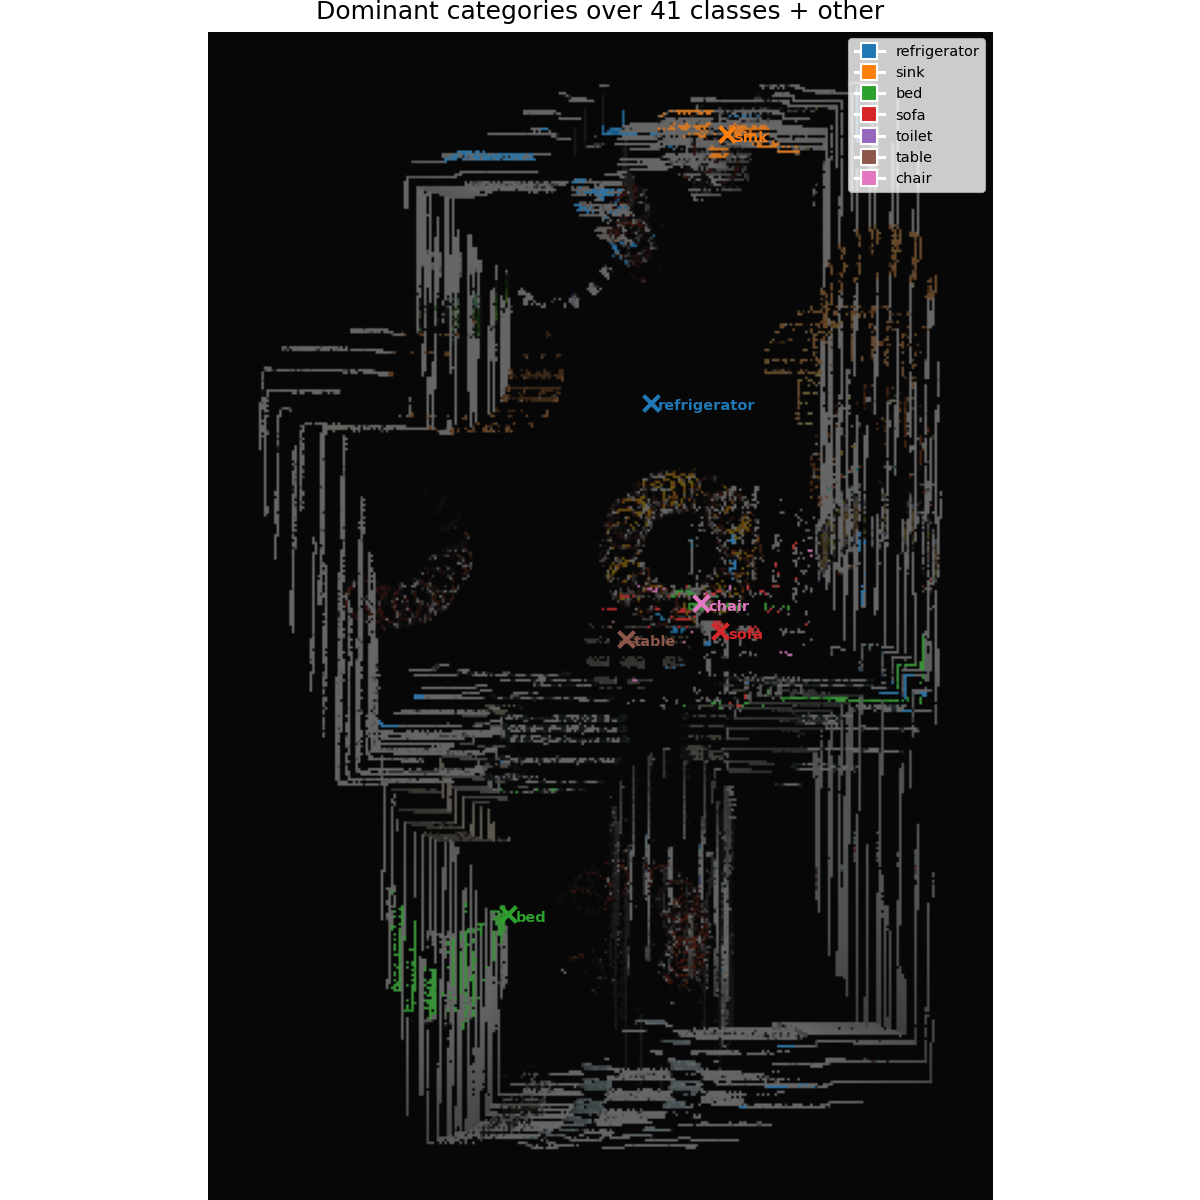
\includegraphics[width=0.48\linewidth]{figs/vlmap_index_small_house.png}
\hfill
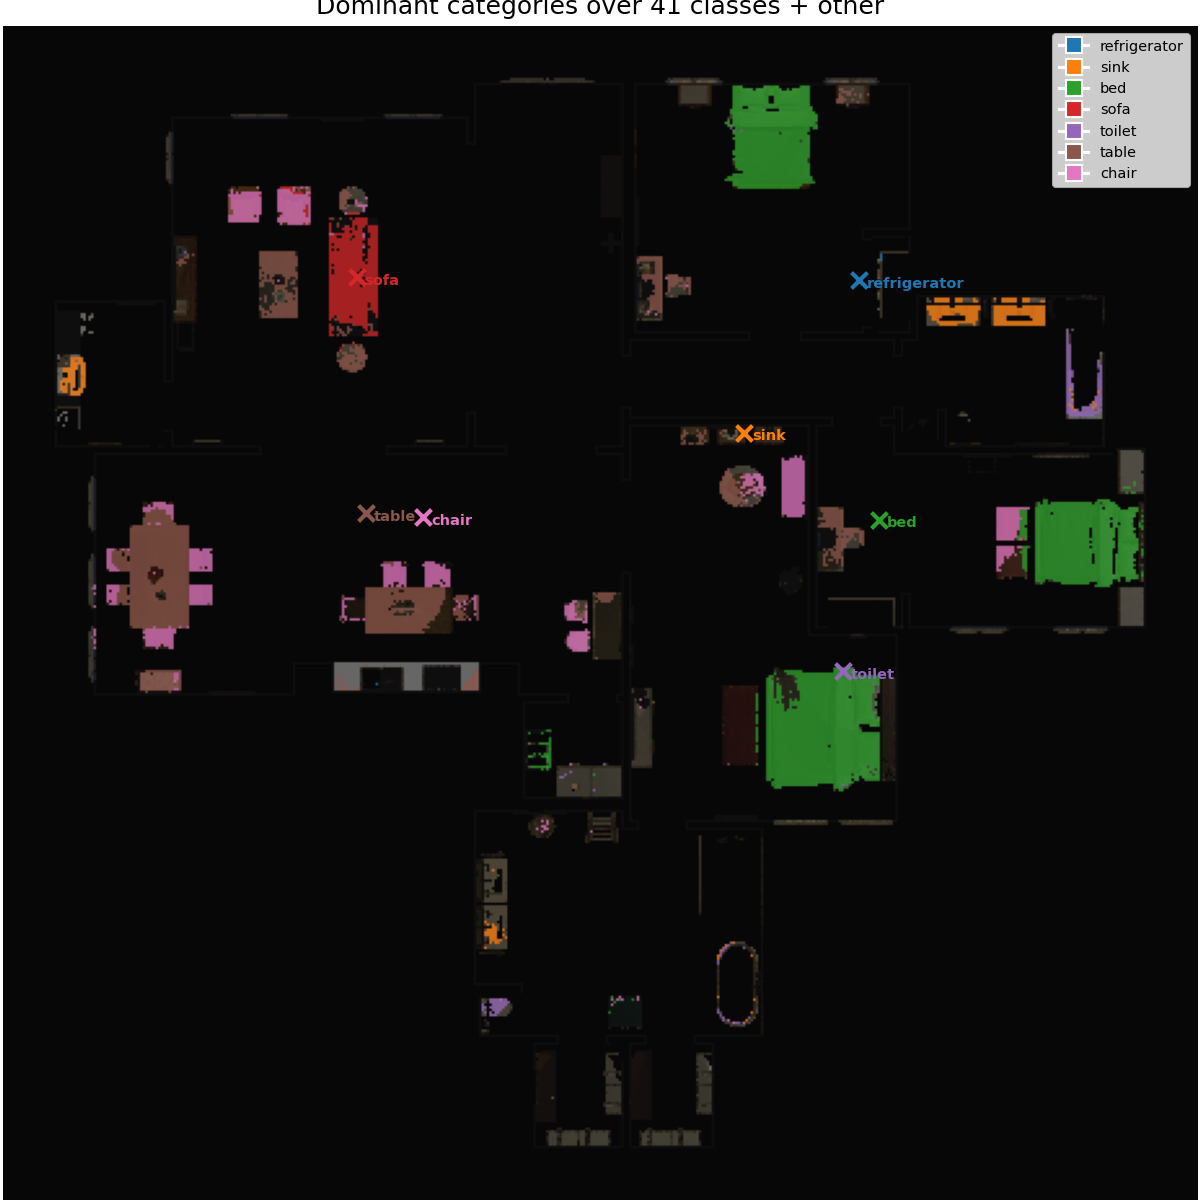
\includegraphics[width=0.48\linewidth]{figs/vlmap_index_hssd_102344280_0.png}
\caption{Resumen dominante por celda para el mapa capturado en
\texttt{small\_house} (izquierda) y para HSSD \texttt{102344280\_0} (derecha).
Cada color representa la categoría que gana el índice multiclase frente al resto
del vocabulario y el fondo.}
\end{figure}

% =============================================================================
\subsection*{24 de abril de 2026}
% =============================================================================

\begin{enumerate}

  \item \textbf{Separación formal de la evaluación en dos fases}: se abandona
        la lectura monolítica del harness 2$\times$2 y se decide evaluar por
        separado (i)~la calidad del heatmap y (ii)~el comportamiento del
        orquestador. El objetivo es aislar causas y poder justificar en la
        memoria del TFG qué parte de la mejora viene del postprocesado del mapa
        semántico y qué parte viene realmente de la política de decisión.

  \item \textbf{Nueva batería \emph{stressed\_heatmap}}: se filtran queries con
        etiquetas como \texttt{multi\_instance}, \texttt{ambiguous\_room} y
        \texttt{explicit\_instance} para forzar escenarios donde el heatmap raw
        produce más picos espurios y el postprocesado debería diferenciarse.
        La batería se expande hasta \textbf{500 queries por escena} para dar
        estabilidad estadística al análisis offline.

  \item \textbf{Resultado de la fase heatmap}: el ganador agregado sobre las
        tres escenas HSSD es \texttt{postprocessed}. No gana por una mejora
        uniforme de todas las métricas geométricas, pero sí en las que mejor
        capturan la utilidad práctica para navegación:
        \begin{itemize}
          \item \texttt{hit@1}: empata en \texttt{102344193\_0} y mejora en
                \texttt{102344280\_0} ($0{,}316 \rightarrow 0{,}414$) y
                \texttt{108736884\_177263634\_4}
                ($0{,}326 \rightarrow 0{,}352$).
          \item \texttt{mass\_in\_expected\_ratio}: mejora en las tres escenas.
          \item \texttt{wrong\_room\_mass\_ratio}: desciende en dos de las tres
                escenas, reduciendo la masa derramada en habitaciones
                incorrectas.
        \end{itemize}
        En cambio, \texttt{hit@5} empeora en dos escenas,
        \texttt{iou\_topmass50} empeora en las tres y
        \texttt{n\_components} permanece estable. La conclusión adoptada es que
        \texttt{Hp} sí merece la pena porque mejora la \emph{hipótesis
        principal}, no porque optimice todas las vistas geométricas del mapa.

  \item \textbf{Nueva batería \emph{stressed\_orchestrator}}: una vez fijado el
        heatmap ganador, se comparan únicamente \texttt{Ob\_Hp} y
        \texttt{Oe\_Hp} sobre queries donde el razonamiento estratégico debería
        importar más. La batería se expande hasta \textbf{100 queries por
        método y escena}.

  \item \textbf{Resultado de la fase orquestador}: el baseline
        \texttt{Ob\_Hp} supera al executor \texttt{Oe\_Hp} en el agregado
        cross-scene del batch estresado:
        \begin{center}
        \begin{tabular}{lcccc}
        \toprule
        \textbf{Método} & \textbf{SR} & \textbf{Wrong Visits} &
        \textbf{Mean Pose Updates} & \textbf{Early Stop Rate} \\
        \midrule
        \texttt{Ob\_Hp} & 0.6667 & 0.1600 & 382.44 & 0.1000 \\
        \texttt{Oe\_Hp} & 0.6167 & 1.1800 & 431.58 & 0.0267 \\
        \bottomrule
        \end{tabular}
        \end{center}
        Aunque el executor mejora algunas métricas intermedias, pierde en las
        métricas principales y además incurre en muchas más visitas erróneas y
        mayor coste de navegación.

  \item \textbf{Configuración base fijada tras la evaluación}: con la evidencia
        reunida hasta esta fecha, la combinación más sólida para seguir
        avanzando pasa a ser:
        \begin{itemize}
          \item heatmap: \texttt{postprocessed},
          \item orquestador: \texttt{baseline},
          \item umbral YOLOE: \texttt{0.30}.
        \end{itemize}
        Esta decisión sustituye a la narrativa previa de ``el executor debería
        ganar'' por una lectura más honesta: el postprocesado aporta valor real
        y el executor, de momento, no justifica su complejidad adicional.

  \item \textbf{Cambio de foco estratégico}: antes de migrar el proyecto a
        ROS\,1, se decide cerrar una capa de semántica abierta sobre HSSD para
        objetos no-VLMap. La idea es validar primero, en simulación controlada,
        un flujo \emph{LLM propone} $\rightarrow$
        \emph{validador filtra} $\rightarrow$
        \emph{YOLOE confirma}, aplicable a objetos concretos como
        \texttt{laptop}, \texttt{book}, \texttt{bottle}, \texttt{teapot},
        \texttt{printer}, etc.

  \item \textbf{Documentación del plan siguiente}: se añade al estado del
        proyecto una nueva etapa intermedia antes de ROS para soportar objetos
        abiertos no presentes en el vocabulario base de VLMaps. La intención es
        endurecer la capa semántica y llegar a la migración con un núcleo más
        maduro, evitando mezclar de golpe problemas de ROS, TF, sensores y
        razonamiento semántico.

\end{enumerate}

\subsection*{14 de abril de 2026}

\begin{enumerate}
  \item \textbf{Reestructuración del documento de proyecto}: se redefine la
        finalidad del proyecto con foco en razonamiento por habitaciones.
  \item \textbf{HSSD confirmado como dataset principal}: MP3D queda como soporte
        secundario; LabelMe diferido.
  \item \textbf{Arquitectura room-aware diseñada}: 8 fases (A--H) con
        representación de estado por habitación, scoring de selección de room,
        acciones de alto nivel y rol estratégico del LLM.
  \item \textbf{Roadmap corregido}: la escalera M1--M5 se reemplaza por la
        arquitectura room-aware como prioridad central. Baselines y evaluación
        pasan a fase posterior.
  \item \textbf{Fase A implementada}: \texttt{SemanticSceneRoomProvider} construido
        con transformación completa Habitat$\rightarrow$grid (\texttt{hab\_to\_grid}).
        Polígonos rasterizados en espacio grid. Cada componente del heatmap anotado
        con su habitación. Navegación a habitación por nombre funcional (centroide
        directo, sin heatmap ni YOLOE). Verificación visual de llegada a habitación
        omitida en simulación (coordenadas exactas); se contempla reactivarla para
        robot real con localización imperfecta.
  \item \textbf{Parsing semántico por niveles}: identificado como trabajo futuro
        necesario. El parsing actual separa instrucciones compuestas en targets
        independientes; se requiere un parser que interprete habitación objetivo +
        objeto dentro de ella como una sola instrucción estructurada.
\end{enumerate}

\subsection*{15 de abril de 2026}

\begin{enumerate}
  \item \textbf{Fase B completada}: \texttt{RoomState} y \texttt{SearchState}
        implementados en \texttt{vlmaps/utils/search\_state.py}. Cada
        \texttt{RoomState} registra \texttt{explored\_ratio}, \texttt{objects\_seen},
        \texttt{candidates\_tried/confirmed}, \texttt{times\_visited},
        \texttt{target\_relevance} y \texttt{target\_found\_here}. Se construye una
        instancia por target al inicio de cada instrucción y se actualiza
        incrementalmente durante la navegación y la verificación YOLOE. Al final de
        cada instrucción se imprime un resumen completo del estado de búsqueda.

  \item \textbf{Fase C completada}: módulo \texttt{vlmaps/utils/room\_priors.py}.
        Implementa \texttt{compute\_room\_priors(query, known\_rooms,
        objects\_seen\_by\_room)} fusionando tres fuentes con pesos
        $a=0{,}5$, $b=0{,}3$, $c=0{,}2$: (a) LLM GPT-4o-mini con llamada
        estructurada al inicio de cada búsqueda de objeto; (b) tabla manual de
        $\sim$35 objetos con scores por tipo de habitación; (c) evidencia de
        co-ocurrencia basada en \texttt{objects\_seen} por habitación. El resultado
        normalizado se almacena en \texttt{RoomState.target\_relevance} y se
        muestra como traza de depuración antes de cada consulta.

  \item \textbf{Navegación solo a candidatos del heatmap}: eliminado el uso de
        \texttt{get\_standoff\_pos()} (que usaba \texttt{labeled\_map\_cropped}).
        Ahora el robot navega directamente al centroide del mejor componente de
        \texttt{kept\_components} (filtrado real por argmax + score $>$ 0{,}3).
        Esto evita que el robot viaje a zonas con señal VLMap pero sin activación
        real en el heatmap.

  \item \textbf{Filtrado de objetos navegables}: la lista de objetos mostrada antes
        de cada consulta usa el mismo filtro que \texttt{compute\_heatmap} (vóxeles
        con argmax ganador y score $> 0{,}3$, mínimo 10 vóxeles), garantizando
        coherencia entre lo que se muestra y lo que el sistema puede encontrar.

  \item \textbf{Correcciones de navegación}: (a) \texttt{n\_actions == 0} tratado
        como ``ya en el destino'' en vez de ``sin camino'', corrigiendo el caso
        post-llegada a habitación; (b) eliminado el bloque de reintento por paso
        estrecho (\textit{narrow-passage retry}) que generaba más falsos positivos
        que beneficios; (c) umbral YOLOE subido a $0{,}3$ y dilatación de obstáculos
        a 3 iteraciones ($\approx$15\,cm por lado).

  \item \textbf{Tipos canónicos de habitación (\textit{room\_type} vs
        \textit{room\_instance})}: HSSD codifica instancias repetidas de un mismo
        tipo de habitación con sufijos numéricos (\texttt{bathroom.001},
        \texttt{bathroom.002}, etc.). Se añade \texttt{canonical\_room\_type()} en
        \texttt{room\_priors.py} que elimina el sufijo \texttt{.NNN} mediante regex
        (\texttt{re.sub(r'\textbackslash.\textbackslash d+\$', '', s)}), y
        \texttt{compatible\_room\_types()} que devuelve el conjunto de tipos
        canónicos con prior $>0{,}05$. Estas funciones permiten razonar sobre
        familias de habitación independientemente del índice de instancia.

  \item \textbf{Comportamiento \textit{local-first} al navegar (\textit{room gate})}:
        nueva función \texttt{select\_best\_candidate(kept\_components, current\_room,
        query\_priors, tried\_centroids)} en \texttt{interactive\_object\_nav.py}. Si
        el robot ya se encuentra dentro de una instancia de habitación cuyo tipo
        canónico es compatible con el objeto buscado (e.g.\ robot en
        \texttt{bathroom.001}, objeto \texttt{sink}), el sistema prioriza los
        candidatos del heatmap situados en esa misma instancia, aplicando un bonus de
        $+0{,}35$ a su calidad efectiva. El cambio de habitación sólo se produce si
        (a) no quedan candidatos locales sin explorar, o (b) la calidad externa supera
        la local en más de un 40\% tras el bonus. El conjunto
        \texttt{\_tried\_centroids} en \texttt{SearchState} registra los centroides ya
        visitados para evitar ciclos.

  \item \textbf{Navegación con margen de seguridad aumentado}: la dilatación de
        obstáculos en \texttt{habitat\_lang\_robot.py} se eleva a 5 iteraciones
        ($\approx$25\,cm por lado). La función
        \texttt{select\_safe\_goal\_from\_path()} aumenta el radio mínimo de
        \textit{clearance} de 3 a 5 celdas y adopta estrategia de máxima holgura:
        reúne \emph{todos} los puntos del camino que cumplen el radio y selecciona el
        de mayor distancia al obstáculo más cercano (en vez del primero válido caminando
        hacia atrás). Si la pasada estricta no devuelve candidatos, una segunda pasada
        suaviza el umbral y vuelve a seleccionar por máxima holgura.

  \item \textbf{Métricas de seguridad por camino}: nueva función
        \texttt{\_compute\_path\_safety(path\_cells, obs\_map)} basada en
        \texttt{distance\_transform\_edt}. Registra longitud, holgura mínima y media,
        penalización acumulada por celdas con $\text{clearance} < 8$ y coste seguro
        $= \text{longitud} + 0{,}5 \cdot \text{penalización}$. Los valores se imprimen
        en trazas \texttt{[safety]} tras cada planificación, facilitando el diagnóstico
        de rutas peligrosas y la futura migración a ROS/HSR.

  \item \textbf{Corrección Bug 1 — comandos de habitación con validación real de
        llegada}: los comandos de tipo \texttt{kitchen}, \texttt{dining room},
        etc.\ fallaban porque el sistema navegaba al centroide geométrico del polígono
        de la habitación (a menudo sobre un obstáculo), el planificador lo desplazaba a
        un nodo visgraph cercano (frecuentemente en otra habitación) y después declaraba
        éxito sin comprobar dónde estaba realmente el robot. Se implementa
        \texttt{find\_reachable\_room\_goal()}, que enumera todas las celdas
        navegables del interior de la habitación objetivo, las ordena por holgura
        respecto a obstáculos y devuelve los top-$K$ candidatos seguros. Tras la
        ejecución del camino se comprueba la habitación real con
        \texttt{get\_room\_at\_cell()} y se valida mediante
        \texttt{\_room\_instance\_matches()}, que acepta tanto coincidencia exacta como
        de tipo canónico (\texttt{kitchen.001} satisface el comando \texttt{kitchen}).
        Si la primera meta falla, se reintenta con los candidatos alternativos antes de
        declarar fracaso. Solo se imprime ``Arrived at room X'' cuando la comprobación
        pasa.

  \item \textbf{Corrección Bug 2 — evidencia del heatmap domina en consultas
        directas}: para consultas de objeto con señal real en el heatmap (p.ej.\
        \texttt{sofa}), los priors de habitación dependían excesivamente de los
        priors lingüísticos (LLM + tabla manual), ignorando que los componentes del
        heatmap ya indicaban en qué habitación está el objeto. Además, nombres de
        habitación específicos de la escena como \texttt{tv} no coincidían con los
        fragmentos estándar (\texttt{living}) de la tabla manual. Se añade la tabla
        \texttt{\_SEMANTIC\_ALIASES} que mapea nombres atípicos a familias semánticas
        (\texttt{tv} $\to$ \texttt{living}, \texttt{laundryroom} $\to$
        \texttt{laundry}, etc.) y se aplica en \texttt{\_manual\_prior()} y
        \texttt{\_evidence\_prior()} mediante \texttt{\_normalize\_room\_for\_priors()}.
        Se añade \texttt{compute\_heatmap\_room\_evidence()} que agrega la calidad de
        componentes por instancia de habitación y normaliza a $[0,1]$. Se extiende
        \texttt{compute\_room\_priors()} con los parámetros opcionales
        \texttt{heatmap\_evidence} y \texttt{query\_type}: las consultas directas usan
        pesos $0{,}65 \cdot \text{heatmap} + 0{,}20 \cdot \text{manual} + 0{,}15
        \cdot \text{LLM}$, mientras que las indirectas mantienen
        $0{,}45 \cdot \text{LLM} + 0{,}30 \cdot \text{manual} + 0{,}25 \cdot
        \text{evidencia escena}$. En el bucle de navegación, tras anotar los
        componentes con su habitación, se recalculan los priors con evidencia real
        antes de seleccionar el candidato, de modo que \texttt{sofa} con tres
        componentes en \texttt{tv} produce un prior $>0{,}86$ para \texttt{tv}.

  \item \textbf{Corrección Bug 3 — puerta de seguridad bloquea ejecución de rutas
        inseguras}: las métricas de seguridad \texttt{[safety]} existían pero eran
        puramente informativas: el sistema ejecutaba igualmente rutas con
        \texttt{goal\_cl=0.0} o \texttt{min\_cl=0.0}. Se añaden umbrales duros
        configurables \texttt{\_MIN\_GOAL\_CLEARANCE=3{,}0} celdas y
        \texttt{\_MIN\_PATH\_CLEARANCE=1{,}0} celdas. Antes de ejecutar cualquier
        camino a un objeto, se evalúan dichos umbrales: si el goal o la ruta no los
        superan, el centroide se marca como intentado en \texttt{\_tried\_centroids}
        y se prueban hasta tres candidatos alternativos. Si ningún candidato
        supera los umbrales, la consulta se omite con mensaje explícito. La
        seguridad ya no es anotación, sino control de flujo.

  \item \textbf{Corrección Problema 1 — metas de aproximación seguras alrededor del
        centroide de componente}: el pipeline anterior planificaba hasta el centroide
        del heatmap (a menudo situado sobre un obstáculo), ejecutaba el camino completo
        y luego recorría el camino hacia atrás buscando un buen punto de observación. Si
        el centroide caía dentro de un obstáculo, el planificador visgraph producía rutas
        erróneas. Se añade \texttt{find\_safe\_candidate\_approach\_goals(centroid,
        safe\_obs\_map, robot\_pos)} que muestrea posiciones de aproximación en un anillo
        de $8$--$25$ celdas alrededor del centroide, filtra por navegabilidad en
        \texttt{\_safe\_obs\_map} y holgura mínima $\ge 3$ celdas, y ordena por holgura
        descendente y proximidad al robot. La meta de navegación se elige directamente
        del mejor candidato del anillo; el camino hacia atrás solo se activa como
        respaldo si el anillo queda vacío.

  \item \textbf{Corrección Problema 2 — planificador global atravesaba paredes}:
        causa raíz doble. (a) La dilatación de obstáculos con 5 iteraciones (bilateral
        $\approx10$ celdas) cerraba los pasillos estrechos de HSSD ($\sim$10 celdas de
        ancho) desconectando habitaciones en el visgraph. Corregido volviendo a
        3~iteraciones ($\approx6$ celdas). (b) El método de recuperación de goal en
        espacio de obstáculo usaba \texttt{G.closest\_point()} (holgura\,=\,0) con
        \texttt{get\_nearby\_position()} como fallback, que devuelve \texttt{None} si
        las cuatro diagonales están bloqueadas; \texttt{vg.Point(None[0])} genera
        coordenadas inválidas $(-1,\,96)$ y \texttt{G.shortest\_path} produce una línea
        recta a través de paredes. Ambas funciones se reemplazan por
        \texttt{\_snap\_to\_nearest\_free(point, obstacles, min\_clearance)} en
        \texttt{navigation\_utils.py}, que usa \texttt{distance\_transform\_edt} para
        encontrar la celda libre más cercana con holgura suficiente: el resultado está
        siempre garantizado dentro del espacio navegable del mapa del visgraph.
        Se añaden también registros de diagnóstico \texttt{[planner] Start navigable:
        \ldots{} Goal navigable: \ldots{}} y almacenamiento del mapa dilatado completo
        como \texttt{robot.\_safe\_obs\_map} para que el resto del sistema use la misma
        referencia que el visgraph. Las funciones
        \texttt{find\_reachable\_room\_goal()} y
        \texttt{find\_safe\_candidate\_approach\_goals()} se actualizan para usar
        \texttt{robot.\_safe\_obs\_map} en lugar del mapa de navmesh crudo, eliminando
        la discordancia entre validación de metas y planificador.

  \item \textbf{Corrección Problema 3 — escudo de colisiones local en ejecución}:
        \texttt{execute\_nav\_replay()} acepta ahora el parámetro opcional
        \texttt{dist\_map} (transformada de distancias del mapa seguro dilatado,
        precalculada una vez antes de cada ejecución). Antes de cada acción
        \texttt{move\_forward}, el escudo predice la siguiente celda de cuadrícula a
        partir de la posición actual \texttt{curr\_pos\_on\_map} y el ángulo
        \texttt{curr\_ang\_deg\_on\_map} del robot. Si la holgura en esa celda es
        inferior a $\texttt{STOP\_CL}\,{=}\,2{,}0$ celdas, la ejecución se interrumpe
        inmediatamente y se activa la recuperación; si la holgura está entre
        $\texttt{STOP\_CL}$ y $\texttt{SLOW\_CL}\,{=}\,5{,}0$ celdas se emite un aviso
        sin detener el movimiento. El escudo opera sobre el mismo mapa dilatado que el
        visgraph, de modo que «celda segura» tiene idéntico significado en planificación
        y en ejecución.

  \item \textbf{Navegación one-shot — eliminados reintentos y recuperación}:
        el escudo de colisiones usaba el mapa dilatado (\texttt{\_safe\_obs\_map})
        para calcular la transformada de distancias, lo que hacía que el centro de
        un pasillo de $\sim10$ celdas tuviera clearance $\approx 2$ en el mapa
        dilatado y disparara paradas falsas al cruzar puertas. El escudo pasa a usar
        \texttt{robot.map.obstacles\_map} (mapa crudo sin dilatar), que refleja el
        espacio físico real; los umbrales se ajustan a
        $\texttt{STOP\_CL}=1{,}0$ y $\texttt{SLOW\_CL}=2{,}5$ celdas.
        Adicionalmente, se elimina la llamada a \texttt{nav\_recovery\_and\_replan()}
        tras un fallo de ejecución y el bucle de reintentos con metas alternativas
        en comandos de habitación. La navegación es ahora estrictamente one-shot:
        se planifica una vez, se ejecuta una vez y se reporta el estado real de la
        habitación; si la ejecución se interrumpe, el robot continúa desde la posición
        actual sin ruta nueva.
\end{enumerate}

% =============================================================================
\subsection*{16 de abril de 2026}
% =============================================================================

\begin{enumerate}

  \item \textbf{Separación explícita entre inflación de planificación y escudo
        de ejecución}: el planificador global utiliza el mapa dilatado
        (\texttt{\_safe\_obs\_map}, 3~iteraciones de dilatación binaria,
        $\approx$15\,cm por lado) para trazar rutas con suficiente margen.
        El escudo de ejecución opera exclusivamente sobre la transformada de
        distancias del mapa crudo (\texttt{robot.map.obstacles\_map}), sin
        dilatar. Esto garantiza que los pasillos estrechos de HSSD
        ($\sim$10~celdas de ancho, clearance real~$\approx$5~celdas) no sean
        bloqueados falsamente por el escudo. La constante
        \texttt{\_PLAN\_DILATION\_ITERS = 3} se declara de forma explícita en
        \texttt{habitat\_lang\_robot.py} y se imprime al inicio de la sesión
        junto con el mensaje: «\textit{global planner only; execution shield
        uses raw map}».

  \item \textbf{Modo de travesía de puertas (\textit{doorway mode})}: antes de
        cada \texttt{move\_forward}, el escudo mide las clearances
        perpendiculares a la derecha y a la izquierda del robot en la pose
        actual (\texttt{\_side\_l}, \texttt{\_side\_r}). Si ambas caen por
        debajo de \texttt{DOORWAY\_SIDE\_TH}~$= 5{,}0$~celdas y la clearance
        frontal supera \texttt{DOORWAY\_FRONT\_MIN}~$= 0{,}5$~celdas, se
        activa el modo de paso estrecho. En ese modo el umbral de parada dura
        se relaja a \texttt{STOP\_CL\_DOOR}~$= 0{,}5$~celdas (frente a
        1{,}0 en espacio abierto) y cada paso se registra como
        «\textit{cautious doorway traversal}». La transición
        ON/OFF se imprime explícitamente. El planificador puede enrutar
        libremente por puertas válidas; el escudo deja cruzarlas sin falsas
        paradas.

  \item \textbf{Escudo sensible a la huella completa del robot}: el chequeo
        anterior solo evaluaba un punto (celda frontal prevista). Ahora se
        evalúan tres puntos de la huella en la pose predicha:
        \textit{front-center}, \textit{front-left} y \textit{front-right}
        (desplazados lateralmente \texttt{ROBOT\_HW}~$= 2$~celdas respecto
        al eje de avance). Se registra por separado
        \texttt{front clearance}, \texttt{left clearance},
        \texttt{right clearance} y \texttt{footprint min clearance}. En
        espacio abierto, si algún lateral cae por debajo de
        \texttt{SIDE\_STOP\_CL}~$= 1{,}5$~celdas, el paso se bloquea. En
        modo puerta, el criterio de bloqueo es solo el mínimo de la huella
        frente a \texttt{DOORWAY\_FRONT\_MIN}.

  \item \textbf{Puerta de entrada a habitación para confirmación YOLOE (\textit{room-entry gate})}: hasta ahora el sistema podía declarar éxito
        inmediatamente si YOLOE detectaba el objeto desde la puerta antes de
        haber cruzado el umbral. Se añade una comprobación en los stages 0
        y~1 de YOLOE: si el robot está en una habitación distinta de la que
        contiene el componente del heatmap objetivo
        (\texttt{best\_comp['room']}) y la distancia al centroide del
        candidato supera 20~celdas ($\approx$1\,m), la detección se marca
        como \textit{tentativa} (\texttt{\_yoloe\_confirmed = False}) y la
        búsqueda continúa con el stage siguiente. Solo se acepta como éxito
        definitivo si el robot ha entrado en la habitación correcta o se
        encuentra a menos de 20~celdas del candidato. Se registra en consola
        «\textit{Object visible but room not yet entered → tentative only}» o
        «\textit{Room entry confirmed}» según el caso.

  \item \textbf{Centrado de trayectorias en pasos estrechos mediante eje medial local}:
        el visgraph seguía generando caminos geométricamente válidos pero
        sesgados hacia uno de los lados del estrechamiento, lo que hacía que el
        escudo de ejecución bloquease pasos por clearance lateral insuficiente
        aun estando en modo de paso estrecho. El primer intento de corrección
        solo recentraba vértices ya existentes y no bastaba cuando el
        estrechamiento caía en mitad de un segmento largo del visgraph. Se
        añade un postprocesado
        \texttt{center\_path\_on\_medial\_axis()} en
        \texttt{vlmaps/utils/navigation\_utils.py}. Tras obtener la ruta del
        visgraph, se rasteriza cada segmento y, si detecta una franja con
        clearance $<4{,}0$ celdas, inserta un waypoint auxiliar en la zona más
        estrecha. Ese waypoint, junto con los intermedios originales, se
        desplaza hacia la celda de mayor holgura dentro de un disco local de
        radio 6, usando \texttt{distance\_transform\_edt} del mapa
        \emph{sin} dilatar. El candidato solo se acepta si mantiene línea de
        visión libre con los waypoints vecino anterior y siguiente sobre el
        mapa de planificación dilatado, evitando atajos que corten esquinas o
        crucen paredes. Después se aplica un suavizado conservador de 3 puntos
        y se conserva la meta final sin desplazar. El resultado es que la ruta
        cruza por el centro del paso incluso cuando el cuello de botella no
        coincide con un vértice del visgraph, y el escudo vuelve a comportarse
        como mecanismo de seguridad, no como corrector sistemático de
        trayectorias.

  \item \textbf{Modo de paso estrecho activado por geometría local, no solo por
        simetría lateral}: en ejecución real aparecía un caso límite al entrar
        oblicuamente en un marco o cuello de botella: un lateral del footprint
        caía por debajo de 1{,}5 celdas mientras el otro seguía aún en espacio
        relativamente abierto, de modo que el detector antiguo no activaba el
        modo de paso estrecho y el escudo bloqueaba el avance con la regla de
        espacio abierto. Se refuerza la detección en
        \texttt{execute\_nav\_replay()} con tres señales:
        (1) estrechamiento en la pose actual, (2) estrechamiento en la huella
        de la pose siguiente y (3) entrada asimétrica, cuando un lateral ya es
        crítico pero la clearance frontal sigue siendo cruzable. Además se
        añade histéresis de salida para mantener el modo activo mientras el
        robot permanezca dentro del cuello de botella. El modo pasa a modelar
        \emph{pasos estrechos cruzables} en general, no solo puertas
        perfectamente simétricas entre habitaciones.

  \item \textbf{Sustitución del \textit{waypoint chasing} por un seguidor de
        polilínea con \textit{lookahead}}: el aumento de waypoints auxiliares
        para centrar la trayectoria en pasos estrechos mejoraba la geometría,
        pero degradaba la ejecución con cientos de micro-correcciones de rumbo,
        porque el controlador discreto original perseguía cada subgoal por
        separado con cuantización fija de 5° y 0{,}1\,m. Se densifica ahora la
        ruta planificada a nivel de celda mediante rasterización de segmentos y
        se ejecuta con un \textit{path follower} sobre esa polilínea densa. En
        cada iteración, el robot proyecta su pose sobre la ruta, selecciona un
        objetivo adelantado (\textit{lookahead}) varios pasos por delante y
        solo aplica la primera acción discreta necesaria para aproximarse a ese
        punto. El \textit{lookahead} se reduce automáticamente dentro de pasos
        estrechos y se mantiene más largo en espacio abierto. Además, las
        métricas de seguridad y la selección de metas de observación pasan a
        evaluarse sobre la misma polilínea densificada, de modo que
        planificación, validación y ejecución comparten por fin la misma
        representación geométrica del camino.

  \item \textbf{\textit{Lookahead} recortado por visibilidad local del camino}:
        el primer seguidor con \textit{lookahead} seguía teniendo un fallo
        importante en pasillos con giro o marcos oblicuos: podía elegir como
        objetivo un punto varios pasos por delante que ya estaba al otro lado
        de una esquina no visible desde la pose actual. Como el controlador
        discreto solo orienta hacia ese objetivo y aplica la primera acción,
        el robot intentaba cortar la esquina y acababa proponiendo un avance
        con \texttt{front clearance = 0.0}. Se corrige haciendo que el
        \textit{path follower} no use directamente el \textit{lookahead}
        preferido, sino el punto más lejano de la polilínea densa que siga
        siendo alcanzable con línea de visión libre sobre el mapa de
        planificación dilatado. Así, dentro de cuellos de botella y giros
        cerrados, el seguidor deja de apuntar ``a través de la pared'' y se
        mantiene sobre el tramo realmente visible del camino.

  \item \textbf{Etiquetas de llegada coherentes con el resultado real de la
        navegación}: en comandos de habitación se estaba mostrando
        ``\textit{Arrived: ...}'' inmediatamente después de que terminara la
        ejecución del follower, incluso si el robot se había detenido antes del
        umbral y la comprobación final de habitación fallaba. Esto inducía a
        error durante la depuración visual. Se corrige la interfaz para que el
        overlay solo muestre ``Arrived'' cuando el robot ha alcanzado de verdad
        la habitación objetivo; en caso contrario, ahora se muestra
        ``Not reached'' en navegación a habitaciones o ``Stopped before goal''
        en aproximaciones a objetos.

  \item \textbf{La referencia de control vuelve a ser la ruta densa, no solo
        la polilínea compactada}: la versión que seguía únicamente la
        polilínea geométrica simplificada seguía permitiendo atajos laterales
        del controlador discreto. En la práctica, el robot podía ``llegar más
        o menos'' al final del segmento pero desviándose del eje real del
        camino, saliéndose hacia paredes o quedándose en la habitación vecina
        cuando el objetivo estaba cerca de una frontera semántica. Se
        reintroduce la trayectoria densa rasterizada como referencia de
        control, pero sin perseguir cada celda individualmente: el follower
        mantiene \textit{lookahead} sobre esa ruta densa y la usa para medir
        progreso y error lateral. La polilínea compactada queda como
        representación del plan, mientras que la ejecución se ancla a la traza
        detallada que realmente debe seguir el robot.

  \item \textbf{Banda muerta angular para eliminar micro-correcciones de 5°}:
        incluso después de volver a seguir la polilínea geométrica, el
        controlador discreto seguía tendiendo a consumir pequeños giros antes
        de casi cada avance cuando el error angular hacia el siguiente objetivo
        era muy bajo. Eso no cambiaba de forma significativa la seguridad, pero
        sí alargaba innecesariamente la ejecución en pasos estrechos. Se añade
        una tolerancia angular en el follower: si el objetivo inmediato ya está
        alineado dentro de un margen moderado, se prioriza
        \texttt{move\_forward} en lugar de corregir rumbo con otro giro
        discreto. La tolerancia es más amplia en zonas estrechas que en espacio
        abierto. Con ello, se reduce el número de pasos y el patrón de
        micro-corrección sin introducir nuevos modos especiales de paso por
        puertas.

  \item \textbf{El shield preventivo se elimina de la ejecución paso a paso}:
        el análisis fino mostró que el escudo local estaba mezclando dos
        nociones incompatibles: clearance sobre un mapa ya dilatado por el
        radio del agente y probes adicionales alrededor del cuerpo. Eso
        generaba falsos bloqueos en puertas y convertía la seguridad en el
        mecanismo principal de decisión, cuando debería ser solo una red de
        protección. La arquitectura actual elimina el \textit{pre-step shield}
        y delega la colisión física en la navmesh de Habitat. La robustez pasa
        a depender de dos piezas más limpias: planificación \textit{clearance-
        aware} y seguimiento fiel del camino.

  \item \textbf{Watchdog de no-progreso real en el follower}: además del fallo
        semántico del shield, aparecía un segundo problema en ejecución: el
        robot podía quedarse vivo cientos de iteraciones repitiendo
        prácticamente la misma pose y agotando el \textit{step budget}. Se
        añade un detector de no-progreso que vigila tanto la celda actual como
        el índice efectivo de progreso sobre la polilínea. Si durante varias
        iteraciones no cambia ni la celda útil ni el progreso útil, la
        ejecución se aborta pronto. También se detecta el caso en que el
        controlador no produce acciones válidas repetidamente para el mismo
        target local. La versión inicial de este watchdog abortaba
        incorrectamente durante la fase de giro en sitio, porque tomaba
        ``misma celda'' como sinónimo de ``sin progreso'' incluso cuando la
        orientación seguía cambiando de forma útil hacia el siguiente tramo del
        camino. Se corrige para que una rotación real también cuente como
        progreso temporal del follower. Con ello, los fallos pasan a ser
        rápidos y diagnosticables en lugar de consumir cientos de pasos
        inmóviles o abortar antes de empezar a avanzar.

  \item \textbf{Reenganche explícito al camino cuando el robot se sale del
        eje}: incluso sin \textit{shield}, el follower seguía pudiendo
        comportarse de forma errática si la banda muerta angular le dejaba
        avanzar cuando ya se había separado lateralmente del trazado. Se añade
        una lógica de \textit{off-track reattachment}: la distancia del robot a
        la ruta densa se mide en cada iteración y, si supera un umbral, el
        \textit{lookahead} se acorta automáticamente para volver a engancharse
        al eje del camino antes de permitir más avance agresivo. Además, la
        banda muerta angular solo puede forzar \texttt{move\_forward} cuando el
        error lateral sigue siendo pequeño.

  \item \textbf{Llegada más estricta en navegación a habitaciones}: la lógica
        anterior consideraba alcanzado el objetivo si el robot quedaba a pocas
        celdas del final del camino. Eso era suficiente para aproximaciones a
        objetos, pero no para comandos de habitación cerca de fronteras
        semánticas: el robot podía detenerse a 1--2 celdas del goal y seguir
        clasificado en la estancia vecina. Se introduce una tolerancia de
        llegada más estricta para navegación a habitaciones, de modo que el
        follower no dé por completado el camino hasta estar realmente encima
        del objetivo final o prácticamente superpuesto a él.

  \item \textbf{Deadband angular menos restrictiva en el follower}: la primera
        versión de la banda muerta angular seguía siendo demasiado conservadora
        porque solo permitía sustituir un giro por un avance si el segundo
        elemento del plan local del controlador ya era \texttt{move\_forward}.
        En la práctica, eso dejaba fuera muchos casos útiles en los que el
        error angular ya era pequeño pero el controlador aún proponía varios
        giros discretos consecutivos. Se elimina esa condición adicional: ahora
        el follower prioriza \texttt{move\_forward} siempre que el error angular
        esté dentro de la tolerancia y la distancia al objetivo inmediato siga
        justificando el avance. Esto reduce el patrón
        ``giro-giro-giro-avance'' en puertas y pasillos angostos sin cambiar la
        arquitectura general del controlador.

\end{enumerate}

% =============================================================================
\subsection*{20 de abril de 2026}
% =============================================================================

\begin{enumerate}

  \item \textbf{Validación en vivo dentro del contenedor de simulación}: en
        lugar de seguir depurando solo con logs pegados manualmente, se pasa a
        ejecutar pruebas reales dentro de \texttt{tfg-sim} sobre la escena
        HSSD usada durante el desarrollo (\texttt{scene\_id=1}). Esto permitió
        comprobar de forma reproducible tres consultas representativas:
        navegación a habitación (\texttt{kitchen}), búsqueda de objeto con
        ambigüedad semántica local (\texttt{sofa}) y búsqueda de objeto con
        varios candidatos plausibles (\texttt{sink}). La prueba en vivo mostró
        que \texttt{kitchen} seguía fallando aunque el \textit{shield} ya no
        bloqueaba puertas, mientras que \texttt{sofa} y \texttt{sink} sí
        llegaban a confirmarse con YOLOE. Con ello quedó claro que el problema
        residual principal ya no estaba en la planificación ni en la
        colisión preventiva, sino en el seguimiento local del camino.

  \item \textbf{Corrección del bucle \texttt{preview produced no action}}:
        el fallo real de \texttt{kitchen} no era una colisión contra paredes,
        sino un colapso del follower cerca de un tramo concreto del camino,
        donde el objetivo local quedaba tan cerca que el controlador discreto
        devolvía repetidamente una previsualización vacía
        (\texttt{progress=58, target=59}). El follower seguía reenganchándose a
        ese mismo índice una y otra vez y acababa abortando sin salir del
        cuello. Se corrige en dos pasos. Primero, el objetivo visible de
        \textit{lookahead} ya no puede ser arbitrariamente cercano salvo cuando
        el robot está realmente desviado o casi en la meta. Segundo, cuando un
        target local sigue produciendo una previsualización vacía, el sistema
        eleva explícitamente un \textit{progress floor} y fuerza al follower a
        no volver a anclarse en ese mismo punto de la ruta. Con este cambio, la
        consulta \texttt{kitchen} deja de abortar en el mismo progreso y
        completa la trayectoria hasta quedar clasificada correctamente dentro de
        la cocina.

  \item \textbf{La calidad semántica del heatmap deja de premiar blobs
        minúsculos}: el caso de \texttt{sofa} reveló otro problema de calidad.
        La fórmula anterior para puntuar componentes del heatmap aún permitía
        que un blob muy pequeño pero extremadamente denso compitiera con una
        región grande correspondiente al sofá real. En la práctica, el robot
        podía priorizar un sillón o una activación residual cercana solo porque
        el componente era compacto, aunque el soporte espacial del sofá fuese
        mucho mayor. Se reformula la \textit{quality} de cada componente para
        favorecer de forma más explícita el soporte semántico real
        (\texttt{sum\_val}) y el tamaño útil del componente, reduciendo el peso
        relativo de activaciones pequeñas. Tras este cambio, en la consulta
        \texttt{sofa} el componente grande asociado al sofá pasa a quedar por
        delante de los blobs minúsculos, evitando que el robot ``vaya al
        sillón'' salvo que semánticamente sea de verdad el mejor candidato.

  \item \textbf{Overlay y visualización más fluidos sin cambiar de backend}:
        también se revisa la parte puramente visual del sistema. El overlay de
        navegación mostraba etiquetas del tipo \texttt{[64/366] -> sofa}, pero
        ese total era poco informativo para el usuario y además enfatizaba lo
        largo que era el seguimiento discreto. Se simplifica el texto en
        pantalla para mostrar solo el paso actual (\texttt{[64] -> sofa}). A
        nivel de fluidez, no se migra al visualizador 3D de Habitat, porque
        eso aumentaría la complejidad sin resolver el cuello principal. En su
        lugar, se mantiene OpenCV y se hace más eficiente: la vista en primera
        persona se sigue actualizando en cada acción, pero el mapa cenital se
        redibuja con una cadencia menor y el retardo explícito por paso se
        reduce prácticamente a cero. Así, la reproducción visual resulta mucho
        más fluida sin penalizar perceptiblemente el rendimiento de la
        simulación ni complicar la arquitectura de depuración actual.

  \item \textbf{Fase D implementada en el pipeline real}: el razonamiento por
        habitaciones deja de ser una traza auxiliar y pasa a intervenir en la
        decisión. Se añade una función \texttt{select\_best\_room()} que, a
        partir de \texttt{SearchState}, la evidencia del heatmap y la posición
        actual del robot, calcula un \texttt{room\_score} por habitación con
        cuatro señales ya disponibles en el sistema: prior semántico, evidencia
        agregada del heatmap, coste BFS sobre el mapa libre y penalización por
        intentos fallidos previos en esa habitación. La habitación ganadora se
        usa inmediatamente para filtrar \texttt{kept\_components} antes del
        ranking fino de candidatos, de modo que el flujo deja de ser
        puramente global. La implementación actual utiliza una proxy práctica
        de \textit{unexplored} basada en visitas y fallos acumulados, y deja
        el seguimiento de cobertura detallada para la futura Fase~F.

  \item \textbf{Ajustes del flujo de búsqueda visual y preparación de tests por
        lote}: tras estabilizar la Fase~D se corrigen varios detalles del flujo
        objeto$\rightarrow$detección. Primero, la selección de goals de
        aproximación deja de aceptar puntos que, aun teniendo clearance y
        perteneciendo a la misma habitación, quedarían geométricamente al otro
        lado de una pared respecto al centroid del candidato; ahora se exige
        además línea libre sobre el mapa de planificación. Segundo, las
        consultas directas a muebles presentes en la escena (por ejemplo
        \texttt{sofa} o \texttt{sink}) dejan de pasar por el \textit{room
        selector}: en ese modo se fuerza una política \textit{nearest-first}
        sobre los candidatos del heatmap y el razonamiento por habitaciones se
        reserva para consultas indirectas o ambiguas. Tercero, cuando la query
        sí activa selección de habitación, se añade un \textit{room stage}
        explícito: el robot navega primero a un goal interior seguro de la sala
        elegida y solo después realiza el acercamiento al candidato concreto,
        evitando verificar desde el centro de una habitación equivocada.
        Cuarto, la confirmación YOLOE pasa a congelar tanto la vista RGB
        anotada como el punto objetivo sobre el mapa cenital, dejando una marca
        persistente de la detección positiva. Finalmente, se preparan scripts
        de \textit{batch testing} para generar automáticamente una batería de
        consultas con todas las habitaciones suficientemente navegables y con
        todos los objetos presentes en la escena, dejando el runtime real de
        esas pruebas para la siguiente ronda de validación manual.

\end{enumerate}

% =============================================================================
\subsection*{21 de abril de 2026}
% =============================================================================

\begin{enumerate}

  \item \textbf{Fase F consolidada y accesible para validación manual}: se da
        por cerrada la capa de acciones de alto nivel introducida el día
        anterior y se revisa explícitamente su alcance real. La implementación
        no modifica todavía el comportamiento \emph{runtime} del robot dentro
        de \texttt{interactive\_object\_nav.py}; su función es preparar la
        transición desde una política \emph{inline} a una política explícita y
        tipada. Quedan definidos cinco tipos de acción
        (\texttt{go\_to\_room}, \texttt{explore\_room},
        \texttt{inspect\_candidate}, \texttt{verify\_target} y
        \texttt{done}), su validación estructural, su serialización JSON para
        la futura capa LLM y un selector de \emph{frontier} intra-habitación
        para \texttt{explore\_room}. En paralelo, \texttt{SearchState} amplía
        su papel como memoria del episodio con un registro ordenado de acciones
        y un rastro de celdas visitadas, que servirán como base del ejecutor de
        la siguiente fase.

  \item \textbf{Pruebas unitarias y acceso desde el menú del contenedor}: para
        que la validación de Fase~F no dependa de Habitat, de la GPU ni de una
        escena concreta, se mantiene una suite \texttt{pytest} autocontenida
        (\texttt{tests/test\_phase\_f\_actions.py}) y, además, se expone su
        ejecución desde el menú interactivo del contenedor mediante una nueva
        opción \texttt{p}. Esta entrada lanza la batería de pruebas de la capa
        de política y muestra de forma inmediata si la representación de
        acciones, el \textit{round-trip} JSON, el registro extendido de
        \texttt{SearchState} y el \textit{frontier picker} siguen siendo
        consistentes. El objetivo aquí no es medir navegación real, sino
        garantizar que la interfaz de alto nivel sobre la que se montará la
        siguiente fase permanece estable antes de conectarla al pipeline
        operativo.

  \item \textbf{Corrección del lanzador de \textit{batch testing}}: al ejecutar
        la opción \texttt{t} del menú con dataset HSSD, el script
        \texttt{tools/nav\_batch\_queries.py} fallaba con
        \texttt{TypeError: string indices must be integers} en
        \texttt{HabitatLanguageRobot.\_\_init\_\_}. La causa era que el script
        cargaba la configuración con \texttt{OmegaConf.load}, que no resuelve
        la lista \texttt{defaults} de Hydra: el campo \texttt{data\_paths}
        quedaba como la cadena literal \texttt{default} en lugar del
        diccionario con \texttt{habitat\_scene\_dir}/\texttt{vlmaps\_data\_dir}.
        Se sustituye la carga manual por \texttt{hydra.compose} con
        \texttt{initialize\_config\_dir}, pasando los \emph{overrides}
        (\texttt{scene\_id}, \texttt{dataset\_type},
        \texttt{scene\_dataset\_config\_file}, \texttt{data\_paths}) por la
        vía oficial de Hydra. Tras el arreglo, el script genera
        \texttt{queries.txt} correctamente y el batch llega a lanzar
        \texttt{interactive\_object\_nav.py}. Queda registrado además que un
        \texttt{scene\_id} fuera de rango (p.\,ej.\ teclear \texttt{11} cuando
        solo existen \texttt{0} y \texttt{1}) provoca un \texttt{IndexError}
        en \texttt{vlmaps\_data\_save\_dirs[scene\_id]}; es una limitación
        de UX del menú, no un bug del pipeline, y se considerará añadir una
        validación previa.

  \item \textbf{Primer corte funcional del executor alternativo}: se materializa
        por fin el apartado ``baseline vs.\ executor'' con una implementación
        inicial real. Se mantiene \texttt{interactive\_object\_nav.py} como
        \emph{baseline} intacto y, en paralelo, se añade
        \texttt{application/interactive\_object\_nav\_executor.py} como nuevo
        entrypoint junto con \texttt{vlmaps/policy/executor.py}. El nuevo
        módulo define un \texttt{ExecutorContext} y un despachador
        \texttt{execute\_action(...)} que traduce las acciones tipadas de
        Fase~F (\texttt{go\_to\_room}, \texttt{explore\_room},
        \texttt{inspect\_candidate}, \texttt{verify\_target},
        \texttt{done}) a comportamiento real reutilizando las primitivas ya
        validadas del baseline: \textit{room staging}, generación de
        \emph{approach goals}, \textit{path replay follower}, chequeos YOLOE
        en llegada y tras giro, \textit{scan}~$360^\circ$ y centrado visual.
        La política de alto nivel se mantiene coherente con el estado del
        proyecto: si la query es una habitación, se genera
        \texttt{go\_to\_room} $\rightarrow$ \texttt{done}; si es un mueble
        directo presente en la escena, se mantiene \textit{nearest-first}
        sin selector de habitación; y para consultas ambiguas o indirectas se
        conserva el flujo jerárquico ``habitación primero, candidato después''.
        Además, el menú del contenedor incorpora una nueva opción
        \texttt{e) Interactive executor navigation}, que permite lanzar esta
        variante sin tocar comandos manuales. La parte \emph{pendiente} ya no
        es construir el ejecutor, sino compararlo sistemáticamente frente al
        baseline con las métricas de Fase~H y con volcados lado a lado del
        heatmap baseline y del heatmap procesado \emph{room-aware}.

  \item \textbf{Resolución explícita de instancias de habitación en el parser y
        en la comprobación de llegada}: se corrige un fallo funcional relevante
        del flujo de navegación por habitaciones. Hasta este punto, órdenes como
        \texttt{bathroom.001} o expresiones más naturales como
        \texttt{bathroom 1} terminaban colapsándose sobre la habitación base
        \texttt{bathroom}, porque el pipeline solo distinguía familias
        semánticas y no instancias concretas. Se introduce un resolvedor
        explícito de nombres de habitación en \texttt{room\_provider.py}, capaz
        de mapear alias amigables
        (\texttt{bathroom 1}, \texttt{bathroom one}, \texttt{bedroom 2}) a sus
        etiquetas exactas de escena (\texttt{bathroom.001},
        \texttt{bedroom.002}, etc.), manteniendo a la vez el comportamiento
        esperado para comandos base como \texttt{bathroom} o \texttt{bedroom},
        que siguen prefiriendo la habitación principal cuando existe. Esta
        resolución se conecta tanto al \emph{baseline} como al nuevo
        \emph{executor}: tras el parse LLM se preservan menciones explícitas de
        instancia presentes en la instrucción original, la selección de
        \emph{room goals} pasa a usar la instancia resuelta y la condición de
        llegada deja de aceptar que \texttt{bathroom} satisfaga
        \texttt{bathroom.001}. Se añade además una batería unitaria nueva
        (\texttt{tests/test\_room\_instance\_resolution.py}) que valida la
        distinción entre habitación base e instancia numerada, junto con la
        compatibilidad con el resto de la capa de acciones de Fase~F.

  \item \textbf{Batería de comparación baseline vs.\ executor disponible desde
        el menú}: el apartado extra deja de ser solo una propuesta en papel y
        pasa a tener una infraestructura operativa para lanzar comparaciones
        controladas. Se añade al menú del contenedor la opción
        \texttt{v) Compare --- baseline vs executor}, que genera un lote común
        de \emph{queries}, ejecuta ambas variantes del navegador sobre ese mismo
        fichero de entrada y resume el resultado en \texttt{CSV} y
        \texttt{markdown}. La implementación queda repartida entre
        \texttt{tools/nav\_batch\_queries.py} (generación del lote),
        \texttt{tools/run\_hssd\_nav\_compare.sh} (orquestación host-side) y
        \texttt{tools/compare\_nav\_runs.py} (resumen query-a-query de
        detecciones, habitación final, abortos y número de actualizaciones de
        pose). No sustituye todavía a la evaluación de Fase~H, pero elimina el
        trabajo manual repetitivo de abrir y comparar logs a mano.

  \item \textbf{Primer corte funcional de Fase~G sobre el executor}: se añade
        \texttt{vlmaps/policy/strategic\_policy.py} como capa de decisión
        estratégica sobre estado estructurado. Esta pieza construye un
        \emph{snapshot} del episodio (prior de habitaciones, evidencia del
        heatmap, shortlist de candidatos, frontiers sugeridos y últimas
        acciones), consulta opcionalmente a un LLM para pedir la siguiente
        \texttt{Action} en formato JSON y valida esa propuesta antes de
        ejecutarla. Si el LLM no está disponible o devuelve una acción
        inconsistente, el sistema cae automáticamente a una política
        heurística determinista, lo que evita romper el flujo ya validado del
        executor. A nivel de integración, \texttt{interactive\_object\_nav\_executor.py}
        deja de preconstruir un plan fijo y pasa a operar como bucle
        ``elegir siguiente acción $\rightarrow$ ejecutar acción'', con modo de
        política seleccionable desde el menú (\texttt{heuristic},
        \texttt{hybrid}, \texttt{llm}). La validación unitaria queda cubierta
        por \texttt{tests/test\_phase\_g\_strategic\_policy.py}.

\end{enumerate}

% =============================================================================
\subsection*{22 de abril de 2026}
% =============================================================================

\begin{enumerate}

  \item \textbf{El \textit{testing} deja de ser una colección de utilidades y
        pasa a ser un flujo único}: se reorganiza por completo el submenú
        \texttt{t} del contenedor para que muestre solo tres opciones visibles:
        \texttt{Generate test set}, \texttt{Compare full 2x2 pipeline} y
        \texttt{Heatmap-only offline analysis}. Las antiguas utilidades
        intermedias (batch baseline aislado, comparación binaria baseline vs.\
        executor, runner JSONL suelto y tests unitarios de F/G) siguen
        existiendo como piezas internas o de desarrollo, pero dejan de ser el
        flujo principal del usuario. La intención es que la evaluación pase a
        ser reproducible y autoexplicativa: elegir escena(s), pulsar, esperar y
        recoger resultados en una carpeta estándar.

  \item \textbf{Selección explícita del tipo de heatmap en runtime}: hasta esta
        fecha, baseline y executor compartían implícitamente
        \texttt{compute\_heatmap()}, lo que impedía montar una comparación 2x2
        limpia sin duplicar entrypoints. Se introduce
        \texttt{VLMAPS\_HEATMAP\_MODE} con dos modos explícitos:
        \texttt{baseline} (heatmap crudo tras proyección 2D + decay, sin
        postproceso) y \texttt{postprocessed} (pipeline actual con
        \texttt{postprocess\_heatmap}). El baseline y el executor imprimen el
        modo activo al arrancar y el valor queda recogido en el
        \texttt{manifest.json} de cada corrida. Además, ambos entrypoints
        emiten ahora al final de cada query un resumen estructurado
        \texttt{[eval-summary] \{...\}} con habitación final, historial de
        habitaciones, número de candidatos inspeccionados/confirmados, rastro
        de acciones y recuento de celdas visitadas. Esta capa permite
        calcular métricas de Fase~H sin depender de \emph{regex} frágiles sobre
        logs textuales.

  \item \textbf{Runner online 2x2 y agregador de métricas completos}: se añaden
        dos herramientas nuevas. La primera,
        \texttt{tools/run\_full\_2x2\_eval.py}, coordina de forma automática las
        cuatro combinaciones \texttt{Ob\_Hb}, \texttt{Oe\_Hb},
        \texttt{Ob\_Hp} y \texttt{Oe\_Hp}, reutilizando
        \texttt{tools/run\_nav\_eval.py} como runner por método. La segunda,
        \texttt{tools/aggregate\_full\_2x2\_eval.py}, consume los cuatro
        manifiestos y genera dos vistas listas para inspección:
        \texttt{compare\_full.csv}/\texttt{.md} (una fila por query) y
        \texttt{aggregate\_metrics.csv}/\texttt{.md} (una fila por método y
        \emph{slice}). Las salidas se agrupan bajo una estructura homogénea:
        \texttt{/workspace/results/eval\_runs/\{timestamp\}/queries/},
        \texttt{pipeline\_2x2/\{scene\}/Ob\_Hb}, \ldots,
        junto con un \texttt{config.json} raíz que describe escenas, semilla,
        política del executor, rutas de queries y métodos corridos.

  \item \textbf{Métricas online ya instrumentadas y \emph{slicing} por
        \texttt{query\_type}/\texttt{tag}}: el agregador 2x2 calcula ya de forma
        reproducible SR, Object~SR, Room~SR, CFR, CT2R,
        Rooms~Before~Success, Inspections~Before~Success, Wrong~Visits,
        Mean~Pose~Updates, Early~Stop~Rate, Final~Room~Accuracy,
        Preview~No~Action~Rate, Path~Stopped~Early~Rate,
        Mean~Executor~Actions y Mean~Room~Transitions. No todas las métricas
        tienen aún el mismo grado de robustez: por ejemplo,
        \texttt{Inspections Before Success} se aproxima como
        \texttt{candidates\_tried - candidates\_confirmed} cuando la query
        termina en éxito, y \texttt{Rooms Before Success} se interpreta como el
        índice de la primera habitación esperada dentro de \texttt{visit\_history}.
        Estas aproximaciones quedan explícitas en el \texttt{Markdown} generado,
        en vez de presentarlas como magnitudes más precisas de lo que el log
        realmente permite.

  \item \textbf{La evaluación offline de heatmaps gana agregación por slices y
        envoltorio estándar}: \texttt{tools/eval\_heatmap\_postprocess.py}
        mantiene la salida \texttt{per\_query.csv}, pero añade un
        \texttt{aggregate\_by\_slice.csv} y tablas adicionales en
        \texttt{summary.md} para resumir el rendimiento del heatmap raw y del
        heatmap postprocesado por \texttt{query\_type} y por \texttt{tag}. Para
        que esta tercera opción del submenú no requiera rutas ni carpetas
        manuales, se añade \texttt{tools/run\_heatmap\_offline\_eval.py}, que
        normaliza la salida bajo
        \texttt{/workspace/results/eval\_runs/\{timestamp\}/heatmap\_offline/}
        y escribe también su propio \texttt{config.json}.

  \item \textbf{Validación rápida sin navegación larga}: se ejecutan únicamente
        comprobaciones ligeras, coherentes con el criterio del proyecto de no
        lanzar desde el asistente corridas largas de simulación sin supervisión
        del usuario. Han pasado \texttt{bash -n} sobre el menú, \texttt{py\_compile}
        de los scripts y entrypoints tocados, una batería \texttt{pytest} nueva
        con manifests sintéticos para el agregador 2x2
        (\texttt{tests/test\_eval\_2x2\_tools.py}) y, además, las suites ya
        existentes de Fase~F, Fase~G y resolución de instancias de habitación
        (26 tests). Con ello queda validado el armazón de evaluación; lo que
        falta a partir de ahora es usarlo sobre escenas y JSONLs reales para
        producir resultados y discutirlos en la memoria.

\end{enumerate}

% =============================================================================
\subsection*{23 de abril de 2026}
% =============================================================================

\begin{enumerate}

  \item \textbf{Limpieza del dataset HSSD}: se reduce el listado de escenas
        disponibles a las tres que se usarán en la evaluación oficial:
        \texttt{102344193\_0}, \texttt{102344280\_0} y
        \texttt{108736884\_177263634\_4}. Las restantes (variantes y dos
        carpetas con nombres corruptos generadas por capturas accidentales de
        \texttt{stderr} durante el \emph{collect}) se eliminan de
        \texttt{data/vlmaps\_dataset\_hssd/}. El menú interactivo refleja ya
        sólo \texttt{scene\_id} 0/1/2.

  \item \textbf{Reversión de la rama room-aware en el harness de evaluación}:
        tras un día con seis métodos
        (orquestador~$\times$~heatmap~$\times$~room-aware) se decide volver al
        2$\times$2 original (\texttt{Ob\_Hb}, \texttt{Ob\_Hp}, \texttt{Oe\_Hb},
        \texttt{Oe\_Hp}). Razón: el switch room-aware no es una variable
        independiente de evaluación sino una decisión arquitectónica del
        executor, y mantenerlo como eje del harness multiplicaba el coste sin
        aportar comparaciones nuevas para el nivel actual (muebles y
        habitaciones). \texttt{tools/eval\_methods.py} y
        \texttt{tools/run\_full\_eval.py} vuelven a la matriz de cuatro celdas.

  \item \textbf{Calibración del umbral de confianza de YOLOE}: se introduce un
        sweep dedicado al verificador visual sin barrer los cuatro métodos del
        2$\times$2. Justificación: el conf-thresh sólo afecta la fase de
        verificación al llegar al candidato; las decisiones de navegación,
        heatmap y selección de habitación son independientes. Por tanto basta
        con barrer un único método (\texttt{Oe\_Hp}) para aislar el efecto del
        umbral.

  \item \textbf{Nueva herramienta \texttt{tools/run\_yoloe\_thresh\_sweep.py}}
        (encargada a Codex). Corre \texttt{run\_nav\_eval.py} repetidamente
        sobre la misma escena y JSONL, una vez por threshold, propagando el
        valor vía \texttt{VLMAPS\_YOLOE\_CONF\_THRESH}. Al terminar, agrega los
        manifests y produce \texttt{compare\_thresh.csv} y
        \texttt{compare\_thresh.md} con una fila por threshold y columnas SR,
        Object~SR, Found~rate, Wrong~visits, CFR, CT2R, Early~Stop~Rate.
        Convive sin tocar el harness 2$\times$2 ni el submódulo \texttt{vlmaps}.

  \item \textbf{Resultado del barrido sobre $\{0.30, 0.40, 0.50, 0.60\}$}
        (escena \texttt{102344193\_0}, 50 queries, método \texttt{Oe\_Hp}):
        $\tau=0.30$ maximiza SR (\textbf{0.82}), Object~SR (\textbf{0.76}) y
        \emph{found rate} (\textbf{0.62}) y minimiza las visitas erróneas
        (\textbf{0.84}). A partir de $\tau=0.40$ la degradación es monótona:
        las visitas erróneas se triplican y la SR cae 16~puntos en $\tau=0.60$.
        La constancia de CFR ($0.18$ en los cuatro runs) confirma que el
        experimento aísla correctamente el verificador y no contamina la
        navegación. Los detalles cuantitativos y la decisión están integrados
        en la subsección \emph{Calibración del umbral de confianza de YOLOE}
        del bloque de testing.

  \item \textbf{Discusión honesta sobre la medición de falsos positivos}:
        durante el análisis se descarta el indicador \emph{FP-proxy} inicial
        (\texttt{found} $\land$ $\neg$\texttt{success} sobre queries
        \texttt{room\_object}). Razones: (i)~el \emph{ground truth} del
        \emph{benchmark} es a nivel de habitación, no de instancia, por lo que
        encontrar una instancia válida del mismo objeto en otra habitación se
        contabiliza erróneamente como falso positivo; (ii)~el agente detiene la
        búsqueda en la primera confirmación, ocultando posibles FPs latentes en
        otras habitaciones; (iii)~con sólo 8 queries \texttt{room\_object} el
        indicador es estadísticamente inservible. Se documenta como limitación
        del banco de evaluación que una medición directa de FPs requeriría
        \emph{queries negativas} (objetivo ausente en la escena) o
        \emph{ground-truth} de instancia.

  \item \textbf{Decisión adoptada}: se mantiene $\tau=0.30$ como umbral de
        confianza para todos los métodos del 2$\times$2 oficial. La elección
        queda justificada documentalmente (tabla, gráficos y discusión) en la
        sección de testing, evitando aparecer como un default arbitrario.

  \item \textbf{Decisión estratégica: activar la migración a ROS\,1 Noetic
        antes que el nivel~3}. Tras revisar el coste real de añadir nivel~3
        (objetos pequeños) directamente sobre Habitat y luego portarlo a ROS,
        se concluye que esa secuencia obliga a iterar dos veces sobre los
        mismos componentes (Phase~G, surrogate furniture, YOLOE bridge,
        harness). Se reordena el roadmap para migrar primero el stack a
        ROS\,1 Noetic + Gazebo y desarrollar el nivel~3 directamente sobre el
        stack final. Plazo asumido para la migración completa: \textbf{un mes}
        (hasta el 23~de~mayo de 2026).

  \item \textbf{Renuncia explícita a HSSD como dependencia obligatoria}: las
        escenas pasarán a ser \emph{house worlds} de Gazebo (HSR oficial,
        AWS RoboMaker) o iGibson (15 apartamentos basados en escaneos reales,
        utilizado por MoMa-LLM). El razonamiento por habitaciones, surrogate
        furniture y verificación con YOLOE son agnósticos a la fuente de la
        escena.

  \item \textbf{Esquema de etiquetado de habitaciones por centroides
        + Voronoi} (estilo MoMa-LLM): se sustituye el sistema de polígonos
        \texttt{semantic\_config.json} por una partición de Voronoi sobre
        centroides marcados manualmente (un \emph{click} por habitación). El
        mismo esquema vale para escenas Gazebo, iGibson y, más adelante, para
        el laboratorio físico. Coste de anotación: 5--10 minutos por escena.
        Implementación en \texttt{room\_provider} estimada en una sesión
        manteniendo la interfaz pública.

  \item \textbf{Inspiración explícita en MoMa-LLM} (Honerkamp et~al.,
        RSS SemRob 2024): adopción conceptual de tres ideas del paper, con
        re-implementación propia y \emph{sin copiar código} (compromiso de
        integridad académica). Las ideas adoptadas son: (i)~clustering de
        habitaciones por Voronoi; (ii)~vocabulario de acciones de alto nivel
        (ya parcialmente cubierto por la Phase~F existente); (iii)~métrica
        AUC-E (área bajo la curva de eficiencia) como complemento al SR a
        \emph{budget} fijo, para reportar resultados en la memoria.

  \item \textbf{Continuidad de Docker en host distinto}: la migración mantiene
        Docker como mecanismo de empaquetado. El contenedor pasa de
        \texttt{tfg-sim} (Habitat-Sim sobre Ubuntu~20.04) a un nuevo contenedor
        Noetic+Gazebo sobre Ubuntu~20.04. El usuario sigue trabajando desde su
        host Ubuntu~22.04 sin reinstalar nada en el host. Cuando se traslade el
        proyecto a un equipo nativo Ubuntu~20.04, el contenedor sigue siendo
        válido (ROS nativo en el host se considera optimización opcional, no
        requisito).

\end{enumerate}


\end{document}
